%%%%%%%%%%%%%%%%%%%%%%%%%%%%%%%%%%%%%%%%
% datoteka diploma-FRI-vzorec.tex
%
%POZOR: ta verzija ne producira pdf datoteke v pdf/A formatu
%namenjena je le za nalogo pri Diplomskem seminarju!
%
% vzorčna datoteka za pisanje diplomskega dela v formatu LaTeX
% na UL Fakulteti za računalništvo in informatiko
%
% na osnovi starejših verzij vkup spravil Franc Solina, maj 2021
% prvo verzijo je leta 2010 pripravil Gašper Fijavž
%
% za upravljanje z literaturo ta vezija uporablja BibLaTeX
%
% svetujemo uporabo Overleaf.com - na tej spletni implementaciji LaTeXa ta vzorec zagotovo pravilno deluje
%

\documentclass[a4paper,12pt,openright]{book}
%\documentclass[a4paper, 12pt, openright, draft]{book}  Nalogo preverite tudi z opcijo draft, ki pokaže, katere vrstice so predolge! Pozor, v draft opciji, se slike ne pokažejo!
 
\usepackage[utf8]{inputenc}   % omogoča uporabo slovenskih črk kodiranih v formatu UTF-8
\usepackage[slovene,english]{babel}    % naloži, med drugim, slovenske delilne vzorce
\usepackage[pdftex]{graphicx}  % omogoča vlaganje slik različnih formatov
\usepackage{fancyhdr}          % poskrbi, na primer, za glave strani
\usepackage{amssymb}           % dodatni matematični simboli
\usepackage{amsmath}           % eqref, npr.
\usepackage{hyperxmp}
\usepackage[hyphens]{url}
\usepackage{csquotes}

\usepackage{caption}
\usepackage{graphicx}
\usepackage{float}

\usepackage[pdftex, colorlinks=true,
						citecolor=black, filecolor=black, 
						linkcolor=black, urlcolor=black,
						pdfproducer={LaTeX}, pdfcreator={LaTeX}]{hyperref}

\usepackage{color}
\usepackage{soul}

\usepackage[
backend=biber,
style=numeric,
sorting=nty,
]{biblatex}


\addbibresource{viri.bib} %Imports bibliography file


%%%%%%%%%%%%%%%%%%%%%%%%%%%%%%%%%%%%%%%%
%	DIPLOMA INFO
%%%%%%%%%%%%%%%%%%%%%%%%%%%%%%%%%%%%%%%%
\newcommand{\ttitle}{Analiza stanja digitalizacije slovenskega lovstva}
\newcommand{\ttitleEn}{Analysis of the state of digitalization of slovenian hunting !!}
\newcommand{\tsubject}{\ttitle}
\newcommand{\tsubjectEn}{\ttitleEn}
\newcommand{\tauthor}{Urh Rozman}
\newcommand{\tkeywords}{digitalizacija, IT, lovstvo}
\newcommand{\tkeywordsEn}{digitalization, IT, hunting}

%%%%%%%%%%%%%%%%%%%%%%%%%%%%%%%%%%%%%%%%
%	HYPERREF SETUP
%%%%%%%%%%%%%%%%%%%%%%%%%%%%%%%%%%%%%%%%
\hypersetup{pdftitle={\ttitle}}
\hypersetup{pdfsubject=\ttitleEn}
\hypersetup{pdfauthor={\tauthor}}
\hypersetup{pdfkeywords=\tkeywordsEn}

%%%%%%%%%%%%%%%%%%%%%%%%%%%%%%%%%%%%%%%%
% postavitev strani
%%%%%%%%%%%%%%%%%%%%%%%%%%%%%%%%%%%%%%%%  

\addtolength{\marginparwidth}{-20pt} % robovi za tisk
\addtolength{\oddsidemargin}{40pt}
\addtolength{\evensidemargin}{-40pt}

\renewcommand{\baselinestretch}{1.3} % ustrezen razmik med vrsticami
\setlength{\headheight}{15pt}        % potreben prostor na vrhu
\renewcommand{\chaptermark}[1]%
{\markboth{\MakeUppercase{\thechapter.\ #1}}{}} \renewcommand{\sectionmark}[1]%
{\markright{\MakeUppercase{\thesection.\ #1}}} \renewcommand{\headrulewidth}{0.5pt} \renewcommand{\footrulewidth}{0pt}
\fancyhf{}
\fancyhead[LE,RO]{\sl \thepage} 
%\fancyhead[LO]{\sl \rightmark} \fancyhead[RE]{\sl \leftmark}
\fancyhead[RE]{\sc \tauthor}              % dodal Solina
\fancyhead[LO]{\sc Diplomska naloga}     % dodal Solina


\newcommand{\BibLaTeX}{{\sc Bib}\LaTeX}
\newcommand{\BibTeX}{{\sc Bib}\TeX}

%%%%%%%%%%%%%%%%%%%%%%%%%%%%%%%%%%%%%%%%
% naslovi
%%%%%%%%%%%%%%%%%%%%%%%%%%%%%%%%%%%%%%%%  

\newcommand{\autfont}{\Large}
\newcommand{\titfont}{\LARGE\bf}
\newcommand{\clearemptydoublepage}{\newpage{\pagestyle{empty}\cleardoublepage}}
\setcounter{tocdepth}{1}	      % globina kazala

%%%%%%%%%%%%%%%%%%%%%%%%%%%%%%%%%%%%%%%%
% konstrukti
%%%%%%%%%%%%%%%%%%%%%%%%%%%%%%%%%%%%%%%%  
\newtheorem{izrek}{Izrek}[chapter]
\newtheorem{trditev}{Trditev}[izrek]
\newenvironment{dokaz}{\emph{Dokaz.}\ }{\hspace{\fill}{$\Box$}}


%%%%%%%%%%%%%%%%%%%%%%%%%%%%%%%%%%%%%%%%%%%%%%%%%%%%%%%%%%%%%%%%%%%%%%%%%%%%%%%
%% PDF-A
%%%%%%%%%%%%%%%%%%%%%%%%%%%%%%%%%%%%%%%%%%%%%%%%%%%%%%%%%%%%%%%%%%%%%%%%%%%%%%%

%%%%%%%%%%%%%%%%%%%%%%%%%%%%%%%%%%%%%%%% 
% define medatata
%%%%%%%%%%%%%%%%%%%%%%%%%%%%%%%%%%%%%%%% 
\def\Title{\ttitle}
\def\Author{\tauthor, ur5575@fri.uni-lj.si !!}
\def\Subject{\ttitleEn}
\def\Keywords{\tkeywordsEn}

%%%%%%%%%%%%%%%%%%%%%%%%%%%%%%%%%%%%%%%% 
% \convertDate converts D:20080419103507+02'00' to 2008-04-19T10:35:07+02:00
%%%%%%%%%%%%%%%%%%%%%%%%%%%%%%%%%%%%%%%% 
\def\convertDate{%
    \getYear
}

{\catcode`\D=12
 \gdef\getYear D:#1#2#3#4{\edef\xYear{#1#2#3#4}\getMonth}
}
\def\getMonth#1#2{\edef\xMonth{#1#2}\getDay}
\def\getDay#1#2{\edef\xDay{#1#2}\getHour}
\def\getHour#1#2{\edef\xHour{#1#2}\getMin}
\def\getMin#1#2{\edef\xMin{#1#2}\getSec}
\def\getSec#1#2{\edef\xSec{#1#2}\getTZh}
\def\getTZh +#1#2{\edef\xTZh{#1#2}\getTZm}
\def\getTZm '#1#2'{%
    \edef\xTZm{#1#2}%
    \edef\convDate{\xYear-\xMonth-\xDay T\xHour:\xMin:\xSec+\xTZh:\xTZm}%
}

%\expandafter\convertDate\pdfcreationdate 

%%%%%%%%%%%%%%%%%%%%%%%%%%%%%%%%%%%%%%%%
% get pdftex version string
%%%%%%%%%%%%%%%%%%%%%%%%%%%%%%%%%%%%%%%% 
\newcount\countA
\countA=\pdftexversion
\advance \countA by -100
\def\pdftexVersionStr{pdfTeX-1.\the\countA.\pdftexrevision}


%%%%%%%%%%%%%%%%%%%%%%%%%%%%%%%%%%%%%%%%
% XMP data
%%%%%%%%%%%%%%%%%%%%%%%%%%%%%%%%%%%%%%%%  
\usepackage{xmpincl}
%\includexmp{pdfa-1b}

%%%%%%%%%%%%%%%%%%%%%%%%%%%%%%%%%%%%%%%%
% pdfInfo
%%%%%%%%%%%%%%%%%%%%%%%%%%%%%%%%%%%%%%%%  
\pdfinfo{%
    /Title    (\ttitle)
    /Author   (\tauthor, ur5575@student.uni-lj.si)
    /Subject  (\ttitleEn)
    /Keywords (\tkeywordsEn)
    /ModDate  (\pdfcreationdate)
    /Trapped  /False
}

%%%%%%%%%%%%%%%%%%%%%%%%%%%%%%%%%%%%%%%%
% znaki za copyright stran
%%%%%%%%%%%%%%%%%%%%%%%%%%%%%%%%%%%%%%%%  

\newcommand{\CcImageCc}[1]{%
	
\includegraphics[scale=#1]{cc_cc_30.pdf}%
}
\newcommand{\CcImageBy}[1]{%
	
\includegraphics[scale=#1]{cc_by_30.pdf}%
}
\newcommand{\CcImageSa}[1]{%
	
\includegraphics[scale=#1]{cc_sa_30.pdf}%
}

%%%%%%%%%%%%%%%%%%%%%%%%%%%%%%%%%%%%%%%%%%%%%%%%%%%%%%%%%%%%%%%%%%%%%%%%%%%%%%%
%%%%%%%%%%%%%%%%%%%%%%%%%%%%%%%%%%%%%%%%%%%%%%%%%%%%%%%%%%%%%%%%%%%%%%%%%%%%%%%

\begin{document}
\selectlanguage{slovene}
\frontmatter
\setcounter{page}{1} %
\renewcommand{\thepage}{}       % preprečimo težave s številkami strani v kazalu

%%%%%%%%%%%%%%%%%%%%%%%%%%%%%%%%%%%%%%%%
%naslovnica
 \thispagestyle{empty}%
   \begin{center}
    {\large\sc Univerza v Ljubljani\\%
%      Fakulteta za elektrotehniko\\% za študijski program Multimedija
%      Fakulteta za upravo\\% za študijski program Upravna informatika
      Fakulteta za računalništvo in informatiko\\%
      Fakulteta za matematiko in fiziko\\% za študijski program Računalništvo in matematika
     }
    \vskip 10em%
    {\autfont \tauthor\par}%
    {\titfont \ttitle \par}%
    {\vskip 3em \textsc{DIPLOMSKO DELO\\[5mm]         % dodal Solina za ostale študijske programe
%    VISOKOŠOLSKI STROKOVNI ŠTUDIJSKI PROGRAM\\ PRVE STOPNJE\\ RAČUNALNIŠTVO IN INFORMATIKA}\par}%
%    UNIVERZITETNI  ŠTUDIJSKI PROGRAM\\ PRVE STOPNJE\\ RAČUNALNIŠTVO IN INFORMATIKA}\par}%
%    INTERDISCIPLINARNI UNIVERZITETNI\\ ŠTUDIJSKI PROGRAM PRVE STOPNJE\\ MULTIMEDIJA}\par}%
%    INTERDISCIPLINARNI UNIVERZITETNI\\ ŠTUDIJSKI PROGRAM PRVE STOPNJE\\ UPRAVNA INFORMATIKA}\par}%
    INTERDISCIPLINARNI UNIVERZITETNI\\ ŠTUDIJSKI PROGRAM PRVE STOPNJE\\ RAČUNALNIŠTVO IN MATEMATIKA}\par}%
    \vfill\null%
% izberite pravi habilitacijski naziv mentorja!
    {\large \textsc{Mentor}: doc. dr. Rok Rupnik \par}%
    {\vskip 2em \large Ljubljana, \the\year \par}%
\end{center}
% prazna stran
%\clearemptydoublepage      
% izjava o licencah itd. se izpiše na hrbtni strani naslovnice

%%%%%%%%%%%%%%%%%%%%%%%%%%%%%%%%%%%%%%%%
%copyright stran
%%%%%%%%%%%%%%%%%%%%%%%%%%%%%%%%%%%%%%%%
\newpage
\thispagestyle{empty}

\vspace*{5cm}
{\small \noindent
To delo je ponujeno pod licenco \textit{Creative Commons Priznanje avtorstva-Deljenje pod enakimi pogoji 2.5 Slovenija} (ali novej\v so razli\v cico).
To pomeni, da se tako besedilo, slike, grafi in druge sestavine dela kot tudi rezultati diplomskega dela lahko prosto distribuirajo,
reproducirajo, uporabljajo, priobčujejo javnosti in predelujejo, pod pogojem, da se jasno in vidno navede avtorja in naslov tega
dela in da se v primeru spremembe, preoblikovanja ali uporabe tega dela v svojem delu, lahko distribuira predelava le pod
licenco, ki je enaka tej.
Podrobnosti licence so dostopne na spletni strani \href{http://creativecommons.si}{creativecommons.si} ali na Inštitutu za
intelektualno lastnino, Streliška 1, 1000 Ljubljana.

\vspace*{1cm}
\begin{center}% 0.66 / 0.89 = 0.741573033707865
\CcImageCc{0.741573033707865}\hspace*{1ex}\CcImageBy{1}\hspace*{1ex}\CcImageSa{1}%
\end{center}
}

\vspace*{1cm}
{\small \noindent
Izvorna koda diplomskega dela, njeni rezultati in v ta namen razvita programska oprema je ponujena pod licenco GNU General Public License,
različica 3 (ali novejša). To pomeni, da se lahko prosto distribuira in/ali predeluje pod njenimi pogoji.
Podrobnosti licence so dostopne na spletni strani \url{http://www.gnu.org/licenses/}.
}

\vfill
\begin{center} 
\ \\ \vfill
{\em
Besedilo je oblikovano z urejevalnikom besedil \LaTeX.}
\end{center}

% prazna stran
\clearemptydoublepage

%%%%%%%%%%%%%%%%%%%%%%%%%%%%%%%%%%%%%%%%
% stran 3 med uvodnimi listi
\thispagestyle{empty}
\
\vfill

\bigskip
\noindent\textbf{Kandidat:} Urh Rozman\\
\noindent\textbf{Naslov:} Analiza stanja digitalizacije slovenskega lovstva\\
% vstavite ustrezen naziv študijskega programa!
\noindent\textbf{Vrsta naloge:} Diplomska naloga na univerzitetnem programu prve stopnje Interdisciplinarni študij računalništva in matematike \\
% izberite pravi habilitacijski naziv mentorja!
\noindent\textbf{Mentor:} doc. dr. Rok Rupnik\\


\bigskip
\noindent\textbf{Opis:}\\ !!ROK RUPNIK
Besedilo teme diplomskega dela študent prepiše iz študijskega informacijskega sistema, kamor ga je vnesel mentor. 
V nekaj stavkih bo opisal, kaj pričakuje od kandidatovega diplomskega dela. 
Kaj so cilji, kakšne metode naj uporabi, morda bo zapisal tudi ključno literaturo.

\bigskip
\noindent\textbf{Title:} 


\bigskip
\noindent\textbf{Description:}\\
opis diplome v angleščini

\vfill



\vspace{2cm}




%%%%%%%%%%%%%%%%%%%%%%%%%%%%%%%%%%% !! IZBRIŠI %%%%%%%%%%%%%%%%%%%%%%%%%%%%%%%%%%%%%%%%%
% prazna stran
\clearemptydoublepage

% zahvala
\thispagestyle{empty}\mbox{}\vfill\null\it%
\noindent 
Na tem mestu zapišite, komu se zahvaljujete za pomoč pri izdelavi diplomske naloge oziroma pri vašem študiju nasploh. Pazite, da ne boste koga pozabili. Utegnil vam bo zameriti. Temu se da izogniti tako, da celotno zahvalo izpustite.  !!
\rm\normalfont



% prazna stran
\clearemptydoublepage

%%%%%%%%%%%%%%%%%%%%%%%%%%%%%%%%%%%%%%%%
% posvetilo, če sama zahvala ne zadošča :-)
\thispagestyle{empty}\mbox{}{\vskip0.20\textheight}\mbox{}\hfill\begin{minipage}{0.55\textwidth}%
Svoji dragi Alenčici. !!(NE)
\normalfont\end{minipage}

% prazna stran
\clearemptydoublepage
%%%%%%%%%%%%%%%%%%%%%%%%%%%%%%%%%%% !! IZBRIŠI %%%%%%%%%%%%%%%%%%%%%%%%%%%%%%%%%%%%%%%%%


%%%%%%%%%%%%%%%%%%%%%%%%%%%%%%%%%%%%%%%%
% kazalo
\pagestyle{empty}
\def\thepage{}% preprečimo težave s številkami strani v kazalu
\tableofcontents{}


% prazna stran
\clearemptydoublepage

%%%%%%%%%%%%%%%%%%%%%%%%%%%%%%%%%%%%%%%%
% seznam kratic

\chapter*{Seznam uporabljenih kratic}

\noindent\begin{tabular}{p{0.1\textwidth}|p{.50\textwidth}|p{.40\textwidth}}    % po potrebi razširi prvo kolono tabele na račun drugih dveh!
  {\bf kratica} & {\bf angleško}                              & {\bf slovensko} \\ \hline
  {\bf LZS}   & Hunting Association of Slovenia & Lovska zveza Slovenije \\
  {\bf ZGS}   & Slovenia Forest Service & Zavod za gozdove Slovenije \\
  {\bf IT}    & Information Technology & informacijska tehnologija \\
  {\bf LRS}   & Socialist Republic of Slovenia & Ljudska republika Slovenija \\
  {\bf LD}    & hunting family & lovska družina \\
  {\bf LPN}   & special purpose state hunting grounds & lovišča s posebnim namenom \\
  {\bf OZUL}  & Regional Association of Hunting Area Managers & območno združenje upravljavcev lovišč \\
  {\bf LUO}   & hunting management area & lovskoupravljavsko območje \\
  {\bf CIC}   & International Council for Game and Wildlife Conservation & Mednarodni svet za lovstvo in ohranitev divjadi \\
  {\bf RAM}   & Random Access Memory & bralno-pisalni pomnilnik \\
  {\bf LIS}   & hunting information system & lovski informacijski sistem \\
  {\bf SOAP}  & Simple Object Access Protocol & protokol za preprosto izmenjavo objektov \\
  {\bf REST}  & Representational State Transfer & prenos predstavitvenega stanja \\
  {\bf WCF}   & Windows Communication Foundation & osnova za komunikacijo v Windows okolju \\
  {\bf DRO}   & Slovenian Government Cloud & Državni računalniški oblak \\
  {\bf FAQ}   & Frequently Asked Questions  & pogosto zastavljena vprašanja \\
\end{tabular}



% prazna stran
\clearemptydoublepage

%%%%%%%%%%%%%%%%%%%%%%%%%%%%%%%%%%%%%%%%
% povzetek
\addcontentsline{toc}{chapter}{Povzetek}
\chapter*{Povzetek}

\noindent\textbf{Naslov:} \ttitle
\bigskip

\noindent\textbf{Avtor:} \tauthor
\bigskip

%\noindent\textbf{Povzetek:} 
\noindent 

Diplomsko delo se osredotoča na analizo in predloge za izboljšavo informacijskih sistemov slovenskega lovstva.
Opravljeno je analiza trenutnega stanje IT infrastrukture (informacijski sistem Lisjak, aplikacije za pisarniško poslovanje ...) v Lovski zvezi Slovenija in lovskih družinah.
Analiza je bila narejena preko ankete namenjene lovskim družinam in intervjujev članstva Lovske zveze Slovenije ter Zavoda za gozdove Slovenije.
Prispevki diplome so pridobitev mnenja lovskih družin do raznih možnih izboljšav IT infrastrukture, odkrivanje obstoječih problemov pri komunikaciji med Lovsko zvezo Slovenije, predlogi za izboljšanje povezljivosti in integracijo med različnimi informacijskimi sistemi in med lovskimi organizacijami in zunanjimi izvajalci ter predlogi za razvoj specifičnih IT rešitev, prilagojeni potrebam lovskih družin.  

CCA. 100 besed
 (1) kratek opis obravnavanega problema, (2) kratek opis vašega pristopa za reševanje tega problema in (3) (najbolj uspešen) rezultat ali prispevek diplomske naloge. !!

\bigskip

\noindent\textbf{Ključne besede:} \tkeywords.
% prazna stran
\clearemptydoublepage

%%%%%%%%%%%%%%%%%%%%%%%%%%%%%%%%%%%%%%%% IZBRIŠEŠ !! %%%%%%%%%%%%%%%%%%%%%%%%%%%%%%%
% abstract
\selectlanguage{english}
\addcontentsline{toc}{chapter}{Abstract}
\chapter*{Abstract}

\noindent\textbf{Title:} \ttitleEn
\bigskip

\noindent\textbf{Author:} \tauthor
\bigskip

%\noindent\textbf{Abstract:} 
\noindent
The thesis focuses on the analysis and proposals for the improvement of the information systems of Slovenian hunting. An analysis of the current state of IT infrastructure (the Lisjak information system, office applications, etc.) in the Slovenian Hunting Association and hunting families has been carried out. The analysis was conducted through a survey aimed at hunting families and interviews with members of the Slovenian Hunting Association and the Slovenian Forestry Service. The contributions of the thesis are obtaining opinions from hunting families on various possible improvements to the IT infrastructure, identifying existing communication problems between the Slovenian Hunting Association, proposals for improving connectivity and integration between different information systems and between hunting organizations and external contractors, and proposals for the development of specific IT solutions tailored to the needs of hunting families.  !!
\bigskip

\noindent\textbf{Keywords:} \tkeywordsEn.
\selectlanguage{slovene}
% prazna stran
\clearemptydoublepage
%%%%%%%%%%%%%%%%%%%%%%%%%%%%%%%%%%%%%%%% IZBRIŠEŠ !! %%%%%%%%%%%%%%%%%%%%%%%%%%%%%%%###


%%%%%%%%%%%%%%%%%%%%%%%%%%%%%%%%%%%%%%%%%%%%%%%%%%%%%%%%%%%%%%%%%%%%%%%%%%%%%%%%%%%%%%%%%%%%%%%%%%%%%%%%%%%%%%%%%%
\mainmatter
\setcounter{page}{1}
\pagestyle{fancy}



\chapter{Uvod}
\label{start}

\section{Metodologija dela}

Za zbiranje podatkov o obstoječem stanju digitalizacije slovenskega lovstva, so bile uporabljene tri metode.
To so intervjuji, anketa in !! knjižni/interni materiali LZS.
Naprej so bili izvedeni intervjuji s predstavniki raznih komisij LZS preko spleta.
Temu je sledil pregled internih in javnih materialov od LZS ter javnih književnih materialov !!.
Potem ko je bilo pridobljen pregled stanja digitalizacije, je bila zasnovana anonimna anketa na platformi 1KA \cite{1ka}.


\section{Struktura diplome}

V poglavju Lovstvo v Sloveniji je napisan krajši pregled zgodovine lovstva na Slovenskem, dalji opis pa je na voljo v prilogi.
Opisana je tudi trenutna zakonodajna organiziranost lovstva.
Poglavje Obstoječe stanje informacijskega sistema poda analizo trenutnega stanja IT infrastrukture, specifična analiza sistema Lisjak in preostalimi aplikacijami, ki so uporabljena v LZS.
Naslednje poglavje, Analiza intervjujev s predstavniki LZS, vsebuje informacije o načinu izvajanja intervjujev, ter predstavitev informacij dobljenih iz komisij LZS in njenega vodstva.
V poglavju Anketa za ugotavljanje stanja informacijskih sistemov Lovskih družin so razloženi principi s katerimi so bila ustvarjena vprašanja. 
Vsa vprašanja so obrazložena, prikazani so rezultati anketa na vizualno prijazni način in na koncu je podana analiza rezultatov.
V predzadnjem poglavju, Smernice za strategijo digitalizacije, bodo napisani predlogi strategije in smernic za izboljšanje in digitalizacijo informacijskih sistemov v lovstvu, na podlagi pridobljenih informacij.
V Zaključku bo povzetek glavnih ugotovitev in priporočila za morebitne izboljšava ter zaključne misli.

\chapter{Lovstvo v Sloveniji}
\label{zgodovina}

\section{Zgodovina lovstva v Sloveniji}

Lov v Sloveniji sega v mlajši pleistocen, kjer so prvi lovci uporabljali kamnite odkruške.
V mezolitiku so udomačili pse in začeli loviti z lokom in puščicami, medtem ko je lov sčasoma postal sekundaren način pridobivanja hrane.
Rimljani so lov sprva izvajali peš s kopji in psi ter razvili različne tehnike lova, pri čemer je veljalo, da je divjad nikogaršnja lastnina, zato je lahko lovil vsak.\cite{Lov_8_14}
V 6. stoletju, ko so Slovani naselili Slovenijo, je bila zemlja v lasti posameznih družin, lovska pravica pa povezana z zemljiško lastnino.
V fevdalizmu je kralj imel lastnino nad divjadjo, medtem ko so plemiči imeli ekskluzivne lovske pravice na določene vrste divjadi, vendar niso smeli oddajati lovišč v zakup neplemenitim osebam.
Lovski predpisi so urejali pravice in kazni, pri čemer so bili za kršitve predpisane hude kazni, kot so izgon, pranger ali delo na galeji.\cite{Lov_15_34}
Janez Vajkard Valvasor je v drugi polovici 17. stoletja dokumentiral stanje divjadi, gozdov in lova v Sloveniji, kjer so živeli jelenjadi, divji prašiči in zveri, kot so medved, volk in ris, pri čemer so volkovi povzročali škodo kmetom, vključno z napadi na ljudi. 
S cesarskim patentom iz leta 1849 so lastna lovišča obdržali samo lastniki več kot 115 hektarjev, medtem ko so preostala zemljišča postala občinska lovišča, ki so jih občine dajale v zakup na javnih dražbah, z določenimi pravicami in obveznostmi za zakupnike.
Kranjska postava iz leta 1874 je uvedla lovne dobe in prepovedala lov z zankami ter uvajala lovske karte, ki so lovcem omejile lov na določena območja.\cite{Lov_43_55}

\begin{figure}[h!]  
  \centering
  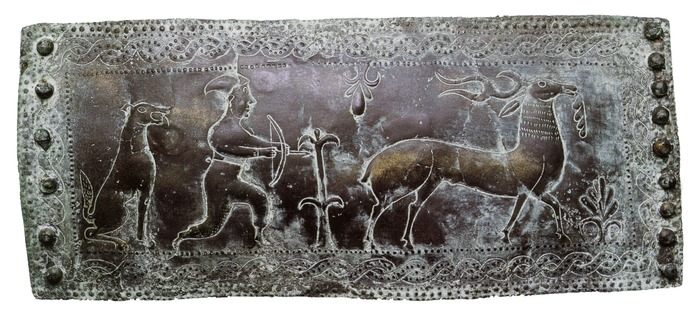
\includegraphics[width=0.8\textwidth]{Bronasta_pasna_spona_iz_Molnika.jpg}  % Adjust the file path as needed
  \caption{Bronasta pasna spona iz Molnika pri Ljubljani (5.stoletje Pr. Kr.) s prizorom psa in lovca \cite{pasna_spona_vir}}
  \label{fig:bronasta_pasna_spona}
\end{figure}

Na dražbah občinskih lovišč so zmagovali bogati posestniki, industrialci, obrtniki in visoki uradniki. 
Posamezniki, ki so želeli imeti pravico do lova, so se združevali v lovske klube in društva, ki so običajno delovala samo za eno zakupno dobo in bila urejena z avstrijskim zakonom iz leta 1867. 
Ta zakon je zahteval prijavo ustanovitve v treh dneh ter posredovanje pravil društva in seznama funkcionarjev.
Dr. Ivan Lovrenčič je leta 1907 predlagal ustanovitev organizacije za vse slovenske lovce, ki bi skrbela za izobraževanje lovcev, razvoj kinologije in zaščito narave. 
Prvi predsednik Slovenskega lovskega kluba je bil ljubljanski župan Ivan Hribar, podpredsednik pa dr. Ivan Lovrenčič. 
Leta 1910 je začelo izhajati glasilo Lovec, vendar je delovanje društva prekinila prva svetovna vojna.\cite{Lov_65_85}

\begin{figure}[h!] 
  \centering
  \includegraphics[width=0.8\textwidth]{Lovec_1910.jpg}
  \caption{Prva naslovnica glasila Lovec iz leta 1910 \cite{bolcina_osebna}}
  \label{fig:lovec_1910}
\end{figure}

Po prvi svetovni vojni so v Sloveniji še vedno veljali avstro-ogrski lovski predpisi, kar je povzročilo zmedo zaradi različnih zakonodaj. 
Razcvet divjega lovstva in pomanjkanje nadzora sta pripeljala do povečanja števila prijavljenega lovsko varstvenega osebja, pogosto družinskih članov lastnikov lovišč. 
Slovensko lovsko društvo se je zavzemalo za učinkovito čuvajsko službo in denarne nagrade za ubito škodljivo divjad.
Leta 1919 so uvedli lovske karte za celotno slovensko ozemlje, vendar so se pojavili nesporazumi zaradi različnih lovskih pravil v Ljubljanski in Mariborski oblasti.
Leta 1931 so z banovinsko odredbo uskladili zakonodajo, vendar je nesoglasje med lovci in sadjarji glede zaščite zajca trajalo do druge svetovne vojne, ko so bile razmere na loviščih slabe.\cite{Lov_93_120}

\begin{figure}[h!] 
  \centering
  \includegraphics[width=0.8\textwidth]{Lovci_med_vojnama.jpg}  % Scale image to 80% of text width
  \caption{Lovci med vojnama\cite{bolcina_osebna}}
  \label{fig:lovci_med_vojnama}
\end{figure}

Med prvo svetovno vojno je veliko članov Slovenskega lovskega društva služilo v vojski. 
Po vojni so se dolžnosti društva povečale zaradi težav z lovstvom, vključno z opustošenimi lovišči, razdrobljeno zakonodajo in razmahom divjega lovstva.
Društvo je začelo ustanavljati podružnice in organizirati sestanke ter predstavitve, vodil pa ga je odbor s predsednikom, podpredsednikom in 25-imi odborniki. 
Najvišji organ društva je bil občni zbor, ki je letno odločal o spremembah pravil, poročilih odbora ter volil vodstvo. 
Mandat odbornikov je bil prvotno enoletni, leta 1926 pa podaljšan na tri leta.
Leta 1924 je društvo postalo razdeljeno na ljubljansko in mariborsko sekcijo, leta 1929 pa je bila zaradi uvedbe banovin združena v Dravski banovini in lovska zveza poenotena.\cite{Lov_129_149}

\begin{figure}[h!]
    \centering
    \captionsetup{skip=5pt}
    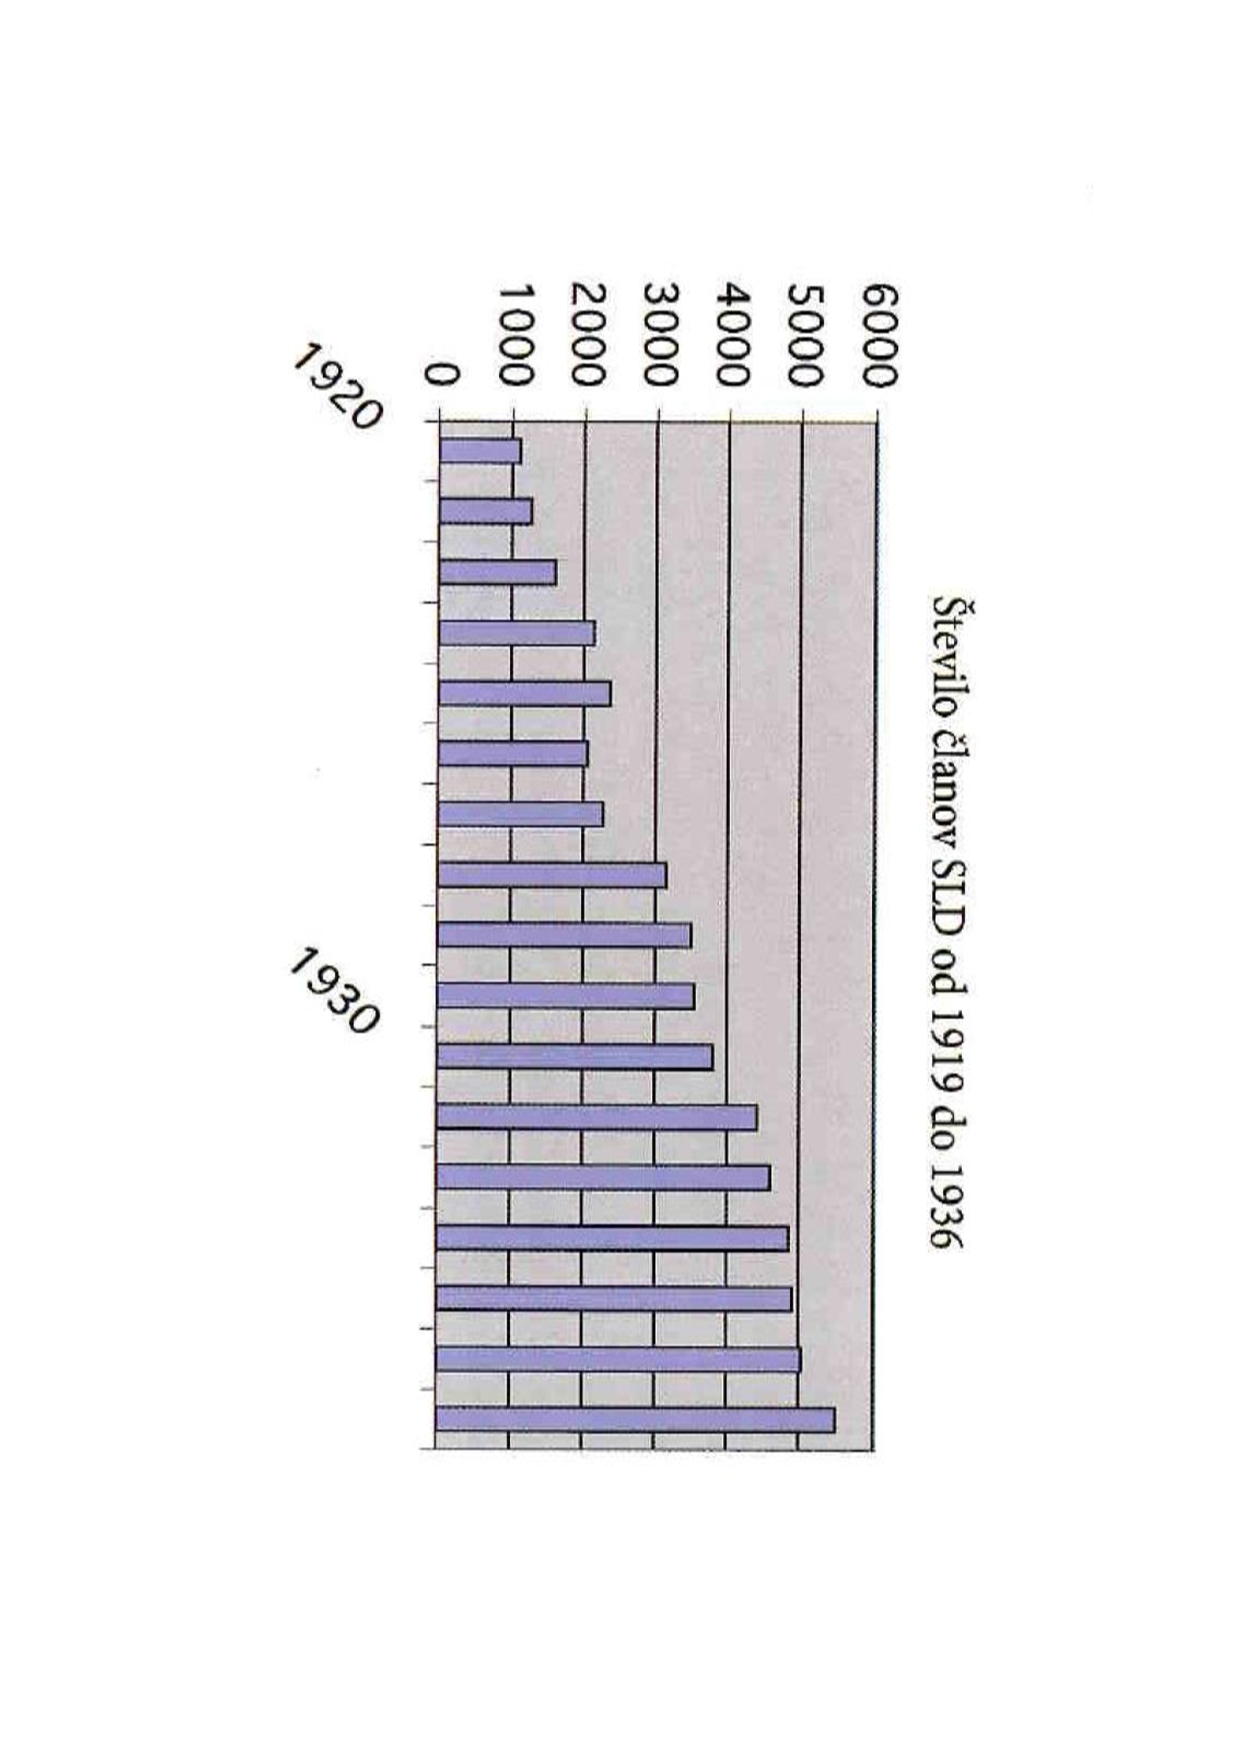
\includegraphics[width=0.5\textwidth, angle=90]{Lov_138_graf_clanstva.png}
    \caption{Graf Članstva SLD \cite[138]{Lov}}
    \label{fig:lov_138}
\end{figure}

Takoj po prvi svetovni vojni so začeli izdajati društveno glasilo Lovec, ki je bilo zaradi svoje kvalitete leta 1921 priporočeno izobraževalnim ustanovam.
Zaradi finančnih težav in visokih stroškov tiskanja glasila so morali večkrat povečevati članarino.
Leta 1922 so v Ljubljani priredili lovsko razstavo s 421 trofejami, sodelovali pa so tudi z drugimi društvi.
Leta 1930 so se udeležili mednarodne razstave v Leipzigu, kjer so prejeli tri odlikovanja.
Leta 1922 so organizirali prve strelske tekme, ki so postale letni dogodek.\cite{Lov_129_149}

\begin{figure}[h!] 
  \centering
  \rotatebox{90}{\includegraphics[width=0.75\textwidth]{dr._W._Krejči_na_strelskem_mestu.jpg}}
  \caption{Dr. W. Krejči na strelske mestu \cite{bolcina_osebna}}
  \label{fig:dr_w_krejci}
\end{figure}

Enotni zakon o lovu iz leta 1935 v Dravski banovini je povezal lovsko pravico z zemljiško lastnino, divjad pa opredelil kot »nikogaršnjo«. 
Zakon je ohranil delitev na lastna in občinska lovišča, določil minimalno velikost in obveznost lastnikov prevzeti enklave občinskih lovišč. 
Razdelil je divjad na zaščiteno z lovopustom, nezaščiteno in zverjad. 
Za lov na nezaščiteno divjad so bile potrebne posebne odobritve, medtem ko so bila lovska društva izključena iz zakupov, ki so lahko trajali do dvanajst let. \cite{Lov_170_175}
Po uvedbi zakona se je zmanjšalo zanimanje za lov in število legalnih lovcev, kar je povzročilo upad lastnih lovišč ter zmanjšanje zakupnin. 
Kljub temu se način delovanja društev ni bistveno spremenil.\cite{Lov_176_178}

Med drugo svetovno vojno so okupacijske oblasti zahtevale obvezno oddajo orožja, lov pa so izvajali predvsem vojaki, medtem ko je bil lov od aprila 1942 prepovedan. 
Leta 1943 in 1944 je na osvobojenem ozemlju začela veljati nova lovska zakonodaja pod vodstvom inž. Franja Sevnika, ki je zagovarjal zakupni sistem zaradi njegovega ekonomskega interesa za vzdrževanje lovišč. 
Pri pripravi povojne zakonodaje so se strinjali, da je lov gospodarsko pomemben, a je treba zaščititi prebivalstvo pred škodo škodljive divjadi in zverjadi.\cite{Lov_197_201}

Odlok o začasnem izvrševanju lova iz leta 1945 je uvedel potrebo po lovski dovolilnici, medtem ko je varstvena zakonodaja ostala predvojna.
Razmišljali so o dolgoročnih rešitvah, kjer bi lovske zadruge postale edini zakupniki lovišč, z omejitvijo na dve lovišči na zadrugo. 
Državna rezervatna lovišča so bila ustanovljena za šport in reprezentanco, medtem ko so bile razglašene denarne nagrade za pokol volkov, katerih sredstva so prihajala iz iztržka od lovskih dovolilnic. 
Leta 1946 je bil sprejet nov zakon, ki je lovišča razdelil na državna, državnorezervatna, zadružna in okrajna, ter ločil divjad na zaščiteno in nezaščiteno. 
Posebna pozornost je bila namenjena zaščiti kmetijskih in gozdnih kultur ter pokončevanju volkov in potepuških psov.\cite{Lov_202_218}
Splošni zakon o lovu iz leta 1947 je veljal za celotno območje Federativne ljudske republike Jugoslavije, kjer so divjad obravnavali kot splošno ljudsko premoženje, lov pa kot gospodarsko panogo. 
Zakon je določal ločitev divjadi na zaščiteno in nezaščiteno ter razdelitev lovišč na državna in lovišča lovskih organizacij, pri čemer so le člani lovskih društev smeli loviti.
Lovska društva so se združevala v podzveze, zveze ljudskih republik, in vse članice so pripadale Glavni lovski zvezi Jugoslavije.\cite{Lov_235_244}

Leta 1949 je Ljudska republika Slovenija sprejela republiški Zakon o lovu, s katerim je prenehal veljati Splošni zakon o lovu. 
Divjad je bila razdeljena na veliko in malo ter zaščiteno in nezaščiteno, minister za gozdarstvo pa je določal lovopust za zaščitene vrste in lahko prepovedal lov za določene vrste.
Volkove, vrane, srake in kune je bilo možno zastrupljati z dovoljenjem okrajnih ljudskih odborov.
Lovišča so bila razdeljena na državna, republiška in lokalna, z obveznostjo vodenja katastrov (kataster - uradni seznam zemljišč s podatki o parcelah \cite{fran}) in določanja lovskih čuvajev. 
Lovske družine so morale izvajati lovske načrte, skrbeti za napredek lovstva in imeti najmanj osem članov, z upoštevanjem pravil lovskega načrta.\cite{Lov_258_276}
Leta 1947 se je Zveza lovskih društev preimenovala v Lovski svet Ljudske republike Slovenije, kjer so vodilne pozicije postopoma prevzeli "preverjeni partijski kadri."
Lovec je leta 1948 ponovno postal uradno glasilo, a je znanje lovcev ostalo slabo, saj je leta 1951 lovski izpit opravilo le 69\% kandidatov.
Leta 1954 se je Lovska zveza Ljudske republike Slovenije preimenovala v Republiško lovsko zvezo, ki je obravnavala konflikte na regionalni ravni. 
Zakon o lovstvu iz leta 1966 je lovstvo opredelil kot športno, gospodarsko in posebno dejavnost, kar je poudarilo potrebo po dolgoročni ohranitvi divjadi.\cite{Sto_63_77}

\begin{figure}[h!]
    \centering
    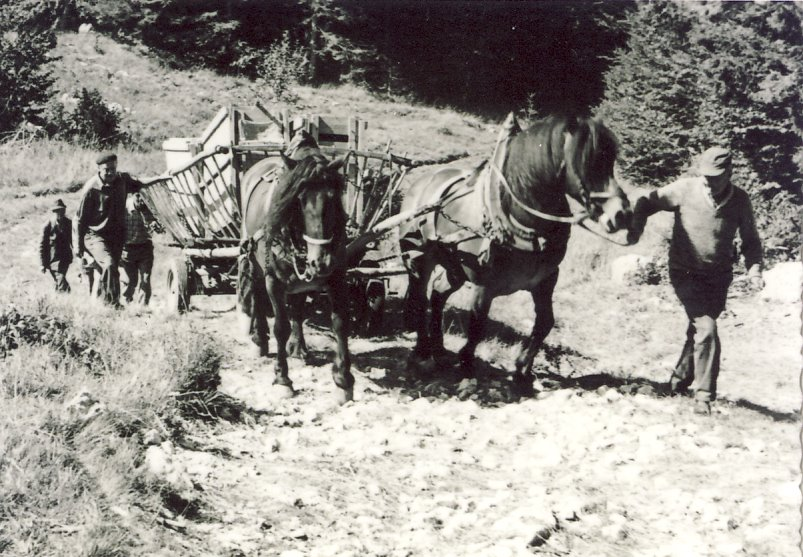
\includegraphics[width=0.7\textwidth]{Naseljevanje_muflonov_1972.png}
    \caption{Naseljevanje muflonov leta 1972 \cite{bolcina_osebna}}
    \label{fig:muflonov_1972}
\end{figure}

V času volitev leta 1990 je Lovska zveza Slovenije poudarila svojo nevtralnost in osredotočenost na lovstvo, med desetdnevno vojno pa je sodelovala s Teritorialno obrambo, kar je povečalo število lovcev v vojaških formacijah. 
Organizacija je pomagala tudi pri diplomatskih aktivnostih, preden je Slovenija postala mednarodno priznana. 
V obdobju 1990-1995 so lovske organizacije prepovedale lov na volkove in predlagale skrajšane lovske dobe za druge vrste.
Leta 1993 so ponovno uvedli občni zbor in odbore ter leta 1998 sprejeli Etični kodeks, ki je določil moralna načela lovcev. 
Nov Zakon o divjadi in lovstvu iz leta 2004 je poudaril varstvo divjadi in ustanovil lovskoupravljalska območja, ki morajo biti večja od 2000 hektarjev, z namenom uravnavanja ravnovesja ekosistema.\cite{Sto_83_104}

\section{Organiziranost lovstva}

Po zakonu so v Republiki Sloveniji edine veljavne lovske organizacije »lovske družine (LD), Lovska zveza Slovenije (LZS), lovišča s posebnim namenom (LPN), javni zavodi ter območno združenje upravljavcev lovišč (OZUL) in lovišč s posebnim namenom, združenih v lovskoupravljavskem območju (LUO)«\parencite[64]{Lov}. 
Krovna organizacija slovenskih lovcev je Lovska zveza Slovenije (LZS), katere članice so lovske družine, lovska društva in ostale organizacije, ki so povezane z divjadjo in varstvom narave oziroma vseh upravljalcev lovišč. 
Temeljni cilji organizacije so skrb za etičnost pri lovu, lovsko kinologijo, zagotavljanje demokratičnih odnosov, sodelovanje z državnimi organi … 

\begin{figure}[h!]
    \centering
    
\includegraphics[width=0.6\textwidth]{logo_LZS.jpg}
    \caption{Logo LZS \cite{bolcina_osebna}}
    \label{fig:logo}
\end{figure}

Konkretne naloge LZS so ozaveščanje lovcev, izvajanje izpitov za lovce, ukvarjanje z razvojem kinologije, izdajanje lovskih izkaznic in sodelovanje pri znanstvenem delu, povezanem z divjadjo. 
Svojim članom nudi strokovno in organizacijsko pomoč. 
LZS se vključuje v mednarodne lovske organizacije, kot na primer CIC oziroma Mednarodni svet za lovstvo in ohranitev divjadi, ki združuje vse lovske organizacije sveta.
Naloge CIC so ohranitev redkih in ogroženih živalskih vrt, spoštovanje globalnega okolja in ustvarjanje partnerskih odnosov lovskih organizacij sosednjih držav.
Lovska družina je društvo, čigar člani so lahko lovci ali pa posamezniki, katerih interes je povezan z divjadjo in lovstvom. 
Po treh letih, ko se je posameznik pridružil lovski družini, je nujno opraviti lovski izpit.
Lovske družine upravljajo z lovišči preko koncesijskih pogodb (koncesija - dovoljenje države tuji trgovski ali industrijski družbi za opravljanje gospodarske dejavnosti na njenem področju \cite{fran}).
Naloge lovskih družin so: zapis evidenc o uplenjenih in najdenih poginulih živali, ocenjevanje škode zaradi divjadi, zbiranje podatkov o divjadi, izvajanje praktičnega dela lovskega izpita … 
Lovišča s posebnim namenom so območja v Republiki Sloveniji, v katerih potekajo specifične naloge s posebnim namenom.
Ustanovljena so bila z Uredbo vlade in so : »Triglav Bled, Kozorog Kamnik, Pohorje, Fazan Beltinci, Kompas Peskovci, Prodi Razor, Jelen, Medved, Snežnik, Kočevska Reka, Žitna gora, Ljubljanski vrh.«\parencite[65]{Lov}
LPN ustanovi Vlada na predlog ministra zaradi posebnih nalog s področja razvoja populacij divjadi. 
Poglavitne naloge LPN so ohranjanje celovitosti in biotske raznovrstnosti lovišč ter divjadi vseh vrst, s tem da se upošteva naravno populacijsko razmerje. 
LPN vsebuje letni načrt, ki določa število odstrela in izgub za posamezne vrste.\cite{Div_63_71}

»Območno združenje upravljavcev se ustanovi zaradi urejanja in usklajevanja skupnih nalog pri upravljanju z divjadjo.«{65}.
»Lovskoupravljavsko območje (LOU) je širša velikopovršinska ekološka celota, na kateri živijo populacije ene ali več vrst divjadi …«\parencite[66]{Lov}. 
LOU je ustvarjen na podlagi ekoloških dejavnikov skupin populacij divjadi, ki živijo na večjem območju. 
Meje določa Vlada na predlog pristojnega ministrstva, tako da se ne bi populacija delila, cilji LOU pa so ohranitev populacije divjadi ter njihovega okolja.

\begin{figure}[h!]
    \centering
    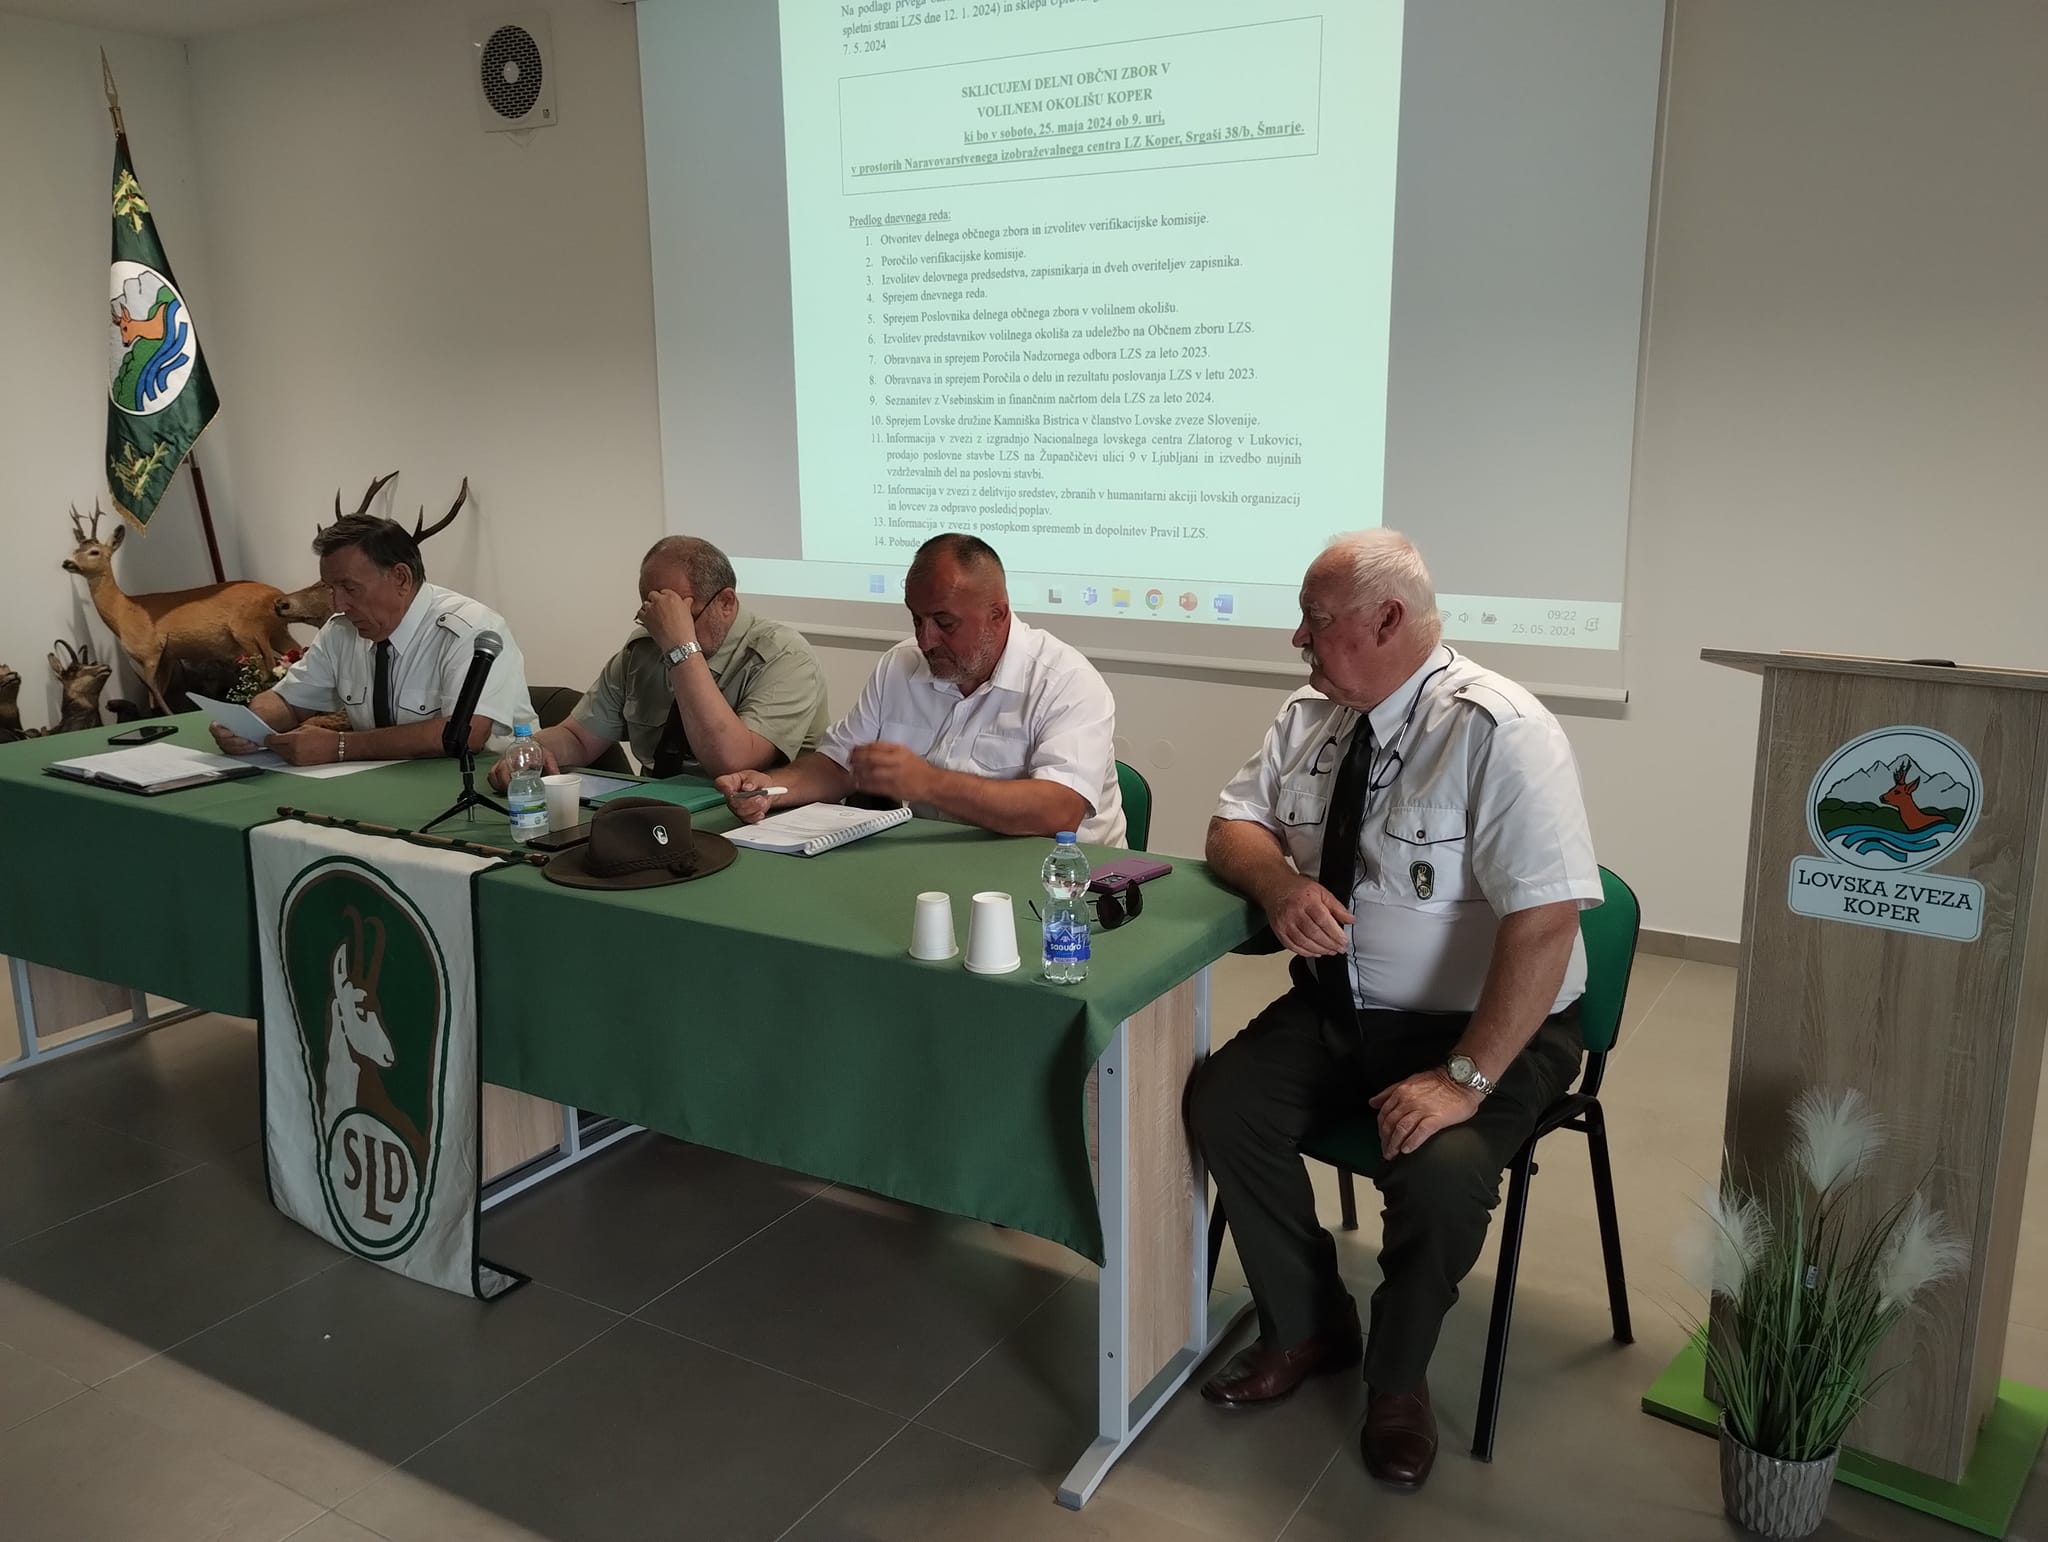
\includegraphics[width=0.6\textwidth]{Delni_obcni_zbor_lzs_LZ_Koper.jpg}
    \caption{Delni občni zbor LZS za volilni okoliš Koper in Občni zbor LZ Koper \cite{LZ_Koper_DOZ}}
    \label{fig:lzs_koper}
\end{figure}



\chapter{Obstoječe stanje informacijskega sistema}
\label{stanje}

\section{IT infrastruktura}

Za vzdrževanje strojne in programske opreme je LZS najela podjetje Artbit.
Eden od obstoječih problemov pri sodelovanju med LZS in tem podjetjem je pomanjkanje izmenjave informacij. 
Večkrat pride do situacij, ko bi lahko težavo predčasno rešili, vendar izvajalci v podjetju Artbit za to prepozno izvejo.
Pojavljajo se tudi težave s strojno opremo, saj se dostikrat zgodi, da so nekateri računalniki članov LZS ali lovskih družin zastareli.
Starejše strojne opreme se ponovno uporabljajo, pri pisarniškem delu pa so zaželeni računalniki z vsaj i5 procesorjem in 8 gigabajtov RAM-a.


\section{Informacijski sistem Lisjak}

Na LZS so leta 2003 sprejeli odličitev o vzpostavitvi informacijskega sistema Lisjak. 
Ta vključuje spletno aplikacijo, zgrajeno po modulih, od katerih so se leta 2005 začeli uporabljati prvi trije moduli, to so članstvo, organizacija in odvzem divjadi.
Obstoječi sistem (po informaciji internega gradiva LZS iz leta 2022, o predstavitvi Lovskega informacijskega sistema (LIS) „Lisjak") vsebuje devet modulov (še lovska škoda in objekti, letni načrt lovišča, izobraževanje, kinologija, delo z mladimi, lovska kultura).
Za odpravo tehničnih težav je sklenjena pogodba z zunanjim izvajalcem.
Strokovne službe LZS, območne lovske zveze, upravljalci lovišč in lovske družine so glavni uporabniki Lisjaka.
Dostop do aplikacije je omogočen samo uporabnikom, ki jo potrebujejo za opravljanje svojih nalog (to so starešine, tajniki, informatiki in strokovni tajniki).
Obstoječih aktivnih uporabnikov je okrog 1700, zaradi zagotavljanja varnosti pa so obvezne menjave gesla na 6 mesecev.
Vsebine modulov so prilagojene spremembam predpisov in pravil, kar omogoča nemoteno delovanje aplikacije.


\section{Aplikacije za pisarniško poslovanje}

Za računovodstvo LZS uporablja storitve podjetja Vasco d.o.o.
Ustanovljeno leta 1991, podjetje razvija programsko opremo za trgovino in računovodstvo, s poudarkom na usklajevanju z zakonodajnimi spremembami. 
Ima 4.000 uporabnikov in ponuja rešitve za manjša in srednje velika podjetja. \cite{vasco}

Za upravljanje z dokumentarnim gradivom v javni upravi LZS uporablja aplikacijo Krpan. 
Ta je nameščen v Državnem Računalniškem Oblaku (DRO), ki nudi uporabnikom shranjevanje. Vključuje več strojnih in programskih komponent in ponuja različne storitve npr. centralna elektronska pošta, hranjenje dokumentov in varnostno kopiranje.\cite{drzavni_oblak}
Krpan uporablja centralne šifrante, kar zagotavlja varnost in učinkovitost upravljanja z dokumenti.
Preko vmesnikov SOAP, REST ali WCF podpira povezave z drugimi informacijskimi sistemi.
Za Krpan veljajo zelo specifične zahteve, saj se vsak uporabnik sistema priključi vladnemu omrežju.\cite{krpan}
V praksi to pomeni, da je potrebno imeti posebno fizično izolirano povezavo do tega omrežja.
S strani LZS so tudi pomisleki o Krpanu, saj je sistem preveč neprilagodljiv.
Za določene postopke je potrebno preveč korakov, zato bi bil bolj primeren enostavnejši sistem. 

Za elektronsko poštvo se uporablja Microsoft 365, ki je nadomestil lastni poštni server LZS.
Velika prednost Microsoft 365 je, da za organizacije, ki pridobijo licenco nevladne organizacije, na voljo brezplačnih 300 e-poštnih računov.
Zunanjim oblikovalcem in lektorjem člani LZS prek elektronske pošte pošiljajo vsebine za glasilo LZS, Lovec.

LZS je lastnik Windows strežnika, ki je pred kratkim prešel na virtualno okolje.
Strežnik je ključnega pomena za posredovanje različnih datotek, predvsem za glasilo Lovec.
Na strežniku je shranjenih skoraj dva terabajta slik.


\section{Ostale aplikacije}

LZS ima adremo (seznam z naslovi, telefonskimi številkami stalnih prejemnikov pošte, sporočil \cite{fran}), s katero spremlja svoje naročnike na revijo. 
Iz letnega poročila LZS za leto 2022 izvemo, da je članov lovskih družin okoli 20.000, zato Excel ni najbolj praktičen.

\section{Integracija z informacijskimi sistemi drugih deležnikov}

Z Zavodom za gozdove Slovenije (ZGS), ki organizirajo LPN (lovišča s posebnim namenom), LZS deli podatke o divjadi posameznih lovskih družin.
Podatke pošiljajo v Excel formatu, ostale pa črpa ZGS iz lovišč za posebne namene preko svojih sistemov. 
Ti pa so zastareli.
Pri ZGS poteka projekt e-gozdarstvo, ki ima za glavno nalogo digitalizacijo vseh področjih gozdarstva, vključno z lovstvom.





\chapter{Analiza intervjujev s predstavniki LZS}
\label{analiza_intervjujev}

Sestanki so potekali od vključno 17. 5. 2024 do vključno 30. 8. 2024. 
Pogovarjali smo se s člani LZS, ki so povezani z delovanjem informacijskega sistema oziroma bi njihovo področje dela bilo lahko izboljšano z uvedbo oziroma vpeljavo informacijskih postopkov.
Intervjuje smo izvedli z naslednjimi člani LZS: s predsednikom Komisije za lovska odlikovanja in priznanja, s predsednikom Komisije za lovsko čuvajsko službo, predsednico Komisije za mlade in lovstvo, s predsednikom Komisije za lovsko kinologijo, z zunanjim izvajalcem za IT, s predstavnikom Zavoda za gozdove Slovenije, s predstavnikom Komisije za izobraževanje in s predsednikom Lovske zveze Slovenije. 

\section{Načina izvajanja intervjujev}

Intervjuji so potekali preko Microsoft Teamsov zaradi več razlogov. 
Člani LZS so lahko izbrali najbolj ustrezen termin, prevoz ni bil potreben in možno je bilo snemanje sestankov.
Ker so bili sestanki posneti, ni bilo treba upočasniti pogovora zaradi izdelave zapiskov.
V povprečju so intervjuji trajali 30 minut.
Vsakemu sogovorniku je bil pred sestankom posredovan sklop točk, tako da so bili seznanjeni s tematiko pogovora in da so se na intervju lahko vnaprej pripravili. 

Struktura pogovora je bila orientirana na naslednje točke:
\begin{enumerate}
    \item Predstavitev komisije
    \item Opis obstoječega stanja digitalizacije pri delovanju komisije
    \item Opis problemov pri delovanju komisije
    \item Priporočila za izboljšavo delovanja komisije v zvezi z digitalizacijo
\end{enumerate}


Najprej je vsak intervjuvanec na kratko predstavil področje komije, njene naloge in odgovornosti. 
Opisano je bilo področje delovanje komisije, vsebina njihovega dela in strokovno znanje, ki je potrebno za delovanje komisije. 
Pri opisu stanja digitalizacije je bil pogovor usmerjen k načinu izvajanja sestankov in urejanju datotek različnih komisij LZS. 
Zanimalo nas je, če sestanki kadarkoli potekajo na daljavo in če, preko katerih kanalov. 
Zanimala nas je organiziranost datotek, ki jih pri svojem delu uporabljajo, kako so formulirane, izpolnjene in shranjene, in če je kakršen koli del procesa avtomatiziran.
V procesu opisovanja stanja so člani LZS pogosto takoj prešli na naslednjo točko pogovora in opisali probleme, ki nastanejo pri postopku delovanja komisij. 
Na koncu smo skupaj oblikovali predloge o izboljšavi delovanja komisij z digitalizacijo. 

\section{Analiza intervjujev s predsedniki komisij}

Prva pogosta opazka v intervjujih je bila, da ni usklajenega načina za izvajanje sestankov. 
Nekatere komisije izvajajo sestanke samo v živo zaradi različnih razlogov in ne na daljavo. 
Eden od razlogov za to je usklajevanje vseh prisotnih na sestankih, saj nekateri starejši člani slabše razumejo digitalno tehnologijo in velikokrat prihaja do težav z uporabo aplikacij za sestanke na daljavo. 
Problem teh sestankov je tudi, da sam sestanek traja dlje časa, saj komunikacija ni takojšnja oziroma prihaja do govorjenja drug čez drugega. 
Še eno nasprotovanje sestankom prek spleta je, da odpade druženje po sestankih, kar pa članom komisij veliko pomeni. 
In zato ima večina članov LZS preferenco za srečanja v živo.
Tiste komisije, ki uporabljajo sestanke na daljavo pa omenjajo prihranke v času, saj so člani sestankov geografsko zelo oddaljeni drug od drugega. 
To je možno pri rednih sejah, kjer je število prisotnih na sestanku manjše in kjer vsi udeleženci znajo uporabljati platforme za videokonference.

Sistem Lisjak je zelo pomemben za izvajanje dela večine komisij znotraj LZS. 
Je platforma, preko katere se vnašajo prijave za kandidate za razna odlikovanja, za podelitev odlikovanj članom lovskih družin, shranjevanje posnetkov predstavitev in predavanj za izobraževanje lovskih čuvajev …
Lisjak uporabljajo komisije bolj kot podatkovno bazo, iz katere jemljejo podatke in jih nato sami preurejajo. 
Večina intervjuvancev je zato priporočila razne možne izboljšave za Lisjaka, ki slonijo na ideji, da bi Lisjak že sam avtomatsko preurejal podatke ali pa da se podatki standardizirajo preden se vnesejo v Lisjak.  
Eden od takih primerov so prijave kandidatov za odlikovanja.
Prijave morajo biti napisane po pravilniku, nato pa so ročno preverjene in ocenjene. 
Če bi Lisjak avtomatično zavrnil nepravilne prijave, ne bi bilo treba preverjati vse prijave ročno in bi se komisija lahko osredotočila na ocenjevanje prijav. 
Naslednji predlog je, da postane pisanje poročil lovskih čuvajev podobno izpolnjevanju podatkovnih baz na Lisjaku.
Obstoječe metode za pisanja poročil so zelo različne, nekateri pišejo še ročno (analogno), drugi pa uporabljajo Microsoft Word.
Možna rešitev, ki je bila omenjena, je avdio posnetek, ki ga nato program pretvori v besedilo. 
Zadnji predlog o Lisjaku, ki je bil omenjen, je ustvarjenje foruma za vsa območja LZS in seznam FAQ oziroma pogosto zastavljena vprašanja na Lisjaku. 
To bi bistveno pomagalo pri zmanjšanju vprašanj, ki jih dobi LZS ter služilo kot kratka predstavitev LZS in njenega delovanja.

\begin{figure}[h!]
    \centering
    \captionsetup{skip=5pt} % Adjust the space between the image and caption
    
\includegraphics[width=0.6\textwidth]{LIS_Lisjak_logo.png}
    \caption{Logo od lovskega informacijskega sistema Lisjak \cite{LIS_Lisjak_logo}}
    \label{fig:lis_lisjak_logo}
\end{figure}

\section{Analiza intervjujev z vodstvom LZS}

Vodstvo LZS je kot enega večjih problemov pri delovanju organizacije omenilo pomanjkanje komunikacije med člani LZS in člani lovskih družin.
Na Lisjaku ni ažuriranih elektronskih naslovov za posamezne lovske družine in drugih kontaktnih podatkov. 
Predlog, ki je bil postavljen za rešitev te dileme je, da bi bila ustvarjena domena lzs.si za elektronsko pošto, kjer bi vsaka lovska družina imela svoj naslov. 

Velika težava pri delu LZS je tudi pomanjkanje arhiviranja podatkov pri nekaterih lovskih družinah. 
Postopek arhiviranja ni enoten, zato je v nekaterih primerih nemogoče ali izredno težko priti do zaželenih podatkov.
Znotraj LZS je uporabljen vladni arhivski sistem Krpan.
Sistem zagotavlja varen zajem in upravljanje digitalnega gradiva ter podpira različne upravne funkcionalnosti s prijaznim uporabniškim vmesnikom.\cite{krpan}
Sistem je dober za arhiviranje in iskanje datotek, omenjena pa je bila časovna zahtevnost za izpolnjevanje nekaterih uradnih dokumentov (npr. potrdil). 
Možno je namreč, da je za izpolnjenje določene datoteke potrebno več oseb. 
To pomeni, da se lahko postopek zaustavi ali zavleče zaradi ene osebe. 

Poudarek pogovora je bil tudi o pomanjkanju informiranja javnosti o dogajanju v lovskih družinah. 
Če javnost ni seznanjena in osveščena o tem kdo so člani organizacije in kaj so njihovi cilji, bodo lovske družine v javnosti slabo sprejete.
Brez informacijske kulture pa ni relevantnih informacij o delu lovskih družin, to pa pomeni, da je težje zagovarjati v javnosti, da so zaupanja vredne organizacije.
Informacije morajo biti pristne, verodostojne in pridobljene v realnem času.
Le s takšnimi podatki je možno izboljšati postopke delovanja lovskih družin na področju informatike.
Potrebna bi bila pravna določba o potrebnosti zbiranja podatkov na relevantnih področjih, nato izobraževanje tajnikov in starešin lovskih družin, da postane zbiranje podatkov učinkovite za potrebe LZS in javnosti.
V intervjujih so bili  posebej omenjeni tajniki, kot najbolj ključni členi lovskih družin, na področju izobraževanja, saj se oni  najbolj ukvarjajo z zbiranjem, urejanjem in filtriranjem podatkov lovskih družin.  

Splošen problem pri izobraževanju odgovornih članov lovskih družin, ki je bil omenjen pri pogovorih, je način prikaza uporabnosti informatike. 
Odlični informacijski sistem je sam po sebi neuporaben, če se člani lovskih družin ne zavedajo ciljev in vrednosti informatike. 
Rečeno je bilo, da morajo biti prikazane otipljive vrednosti, ki so lahko pridobljene, s tem ko se začne sistematizirano zbiranje podatkov. 
Način spremembe kulture lovskih družin o informatiki, se je delno že začelo s prihodom mlajših oseb v organizacije in s povečanjem izobrazbe sedanjih članov.

Obstoječi prihodek mnogih lovskih družin prihajajo od prodaje trofej. 
Vodstvo razmišlja o potencialnih novih ali dodatnih storitvah, ki bi razširilo delovanje lovskih družin. 
Eden od takih predlogov je bila možnost fotografiranja med lovom. 
S tako uporabo informacijskega sistema, bi bila lahko zgrajena podatkovna baza kot osnova za analizo trga, kar bi omogočilo fokusirane storitve in povečanje dobičkov. 

\begin{figure}[h!]
    \centering
    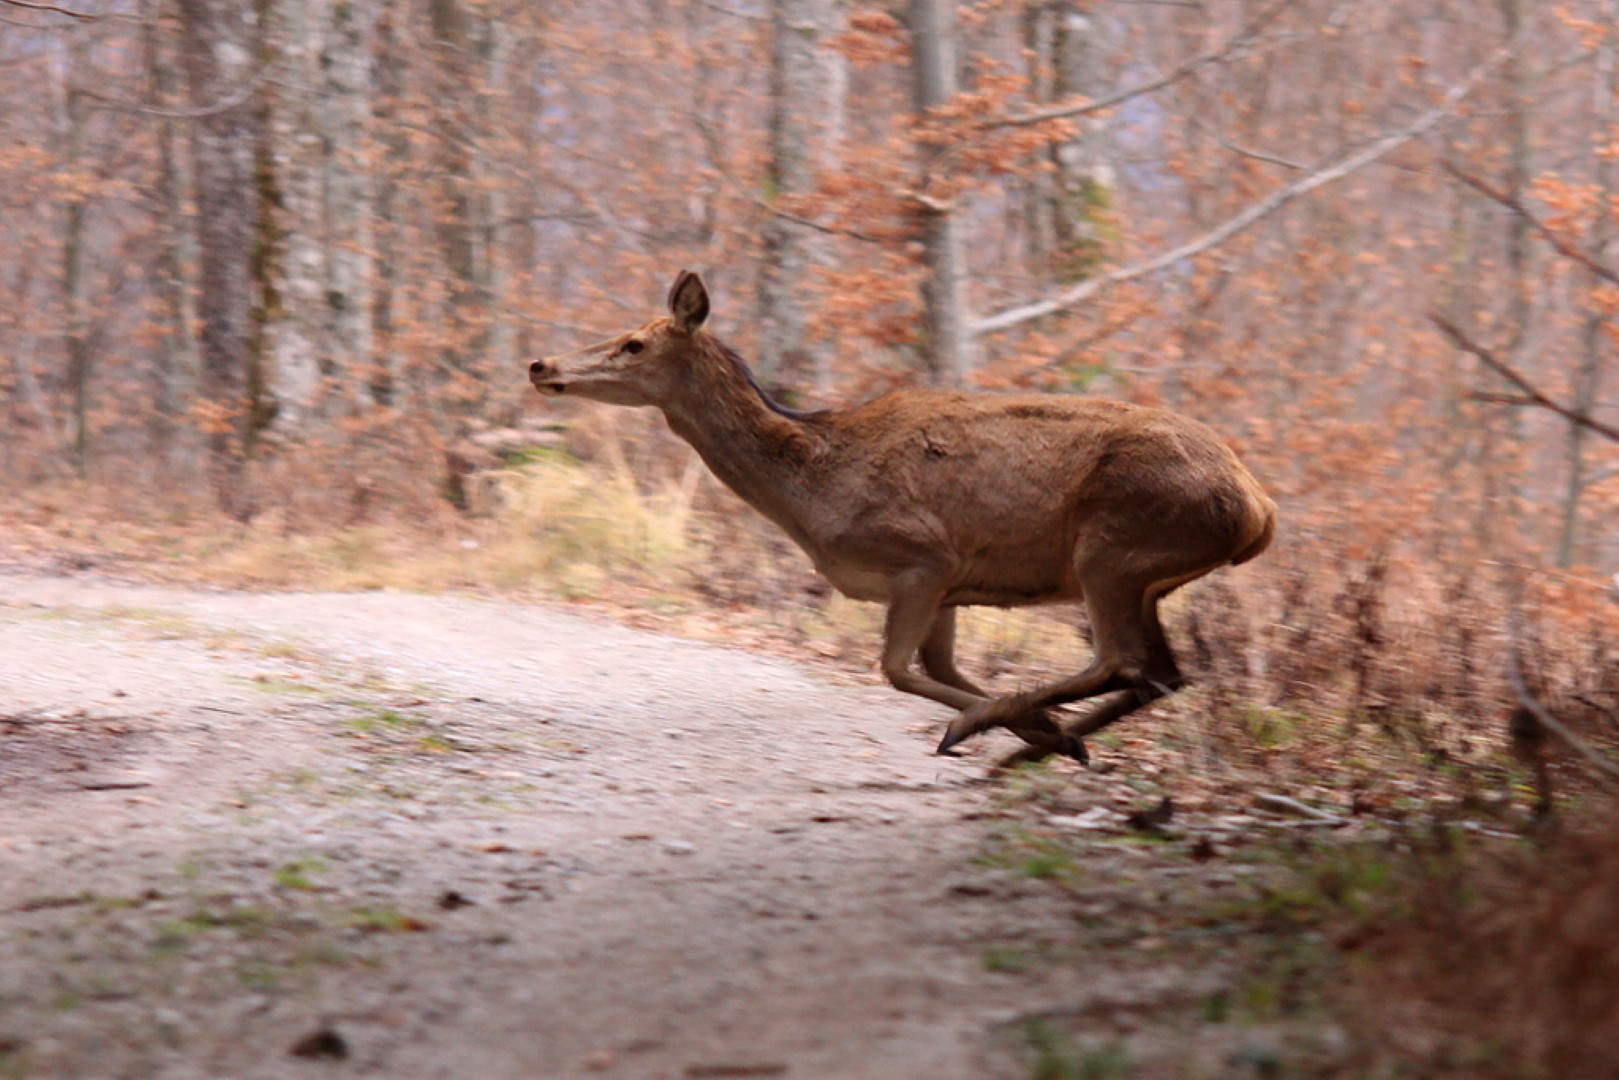
\includegraphics[width=0.7\textwidth]{fotolov_LD_Grosuplje.jpg}
    \caption{Fotolov LD Grosuplje \cite{LD_Grosuplje_fotolov}}
    \label{fig:ld_grosuplje}
\end{figure}




\chapter{Anketa za ugotavljanje stanja informacijskih sistemov Lovskih družin}
\label{anketa}

\section{Zasnova ankete in anketnih vprašanj}

Anketna vprašanja so bila zasnovana na spletni strani 1KA, anketiranje pa je potekalo preko spleta.
Razvija jo Center za družboslovno informatiko na Fakulteti za družbene vede Univerze v Ljubljani.
1KA je odprtokodna aplikacija, katere osnovno vodilo je minimiziranje števila klikov. \cite{1ka}

Vprašanja so bila vezana na mnenja lovskih družin kot organizacij.
Zaželjeno je bilo, da bi za vsako lovsko družino bila izpolnjena natanko ena anketa, da se podatki ne bi podvajali.
Pri izdelavi ankete so bila upoštevana določena načela.
Prvič, anketa ne sme trajati dlje kot 5 minut, saj je zaželjeno učinkovito, hitro izpolnjevanje.
Poleg tega je cilj, da bi čim bolj zmanjšali število anketirancev, ki ne dokončajo ankete.
Drugič, pri vprašanjih, kjer anketiranci izražajo svoja mnenja (za ali proti), ni podana nevtralna možnost, saj je zaželjeno, da se anketiranci maksimalno opredelijo za eno ali drugo možnost.
Tretjič, vprašanja morajo biti oblikovana na način, ki je razumljiv in jasen tudi tistim, ki nimajo poglobljenega znanja o IT zadevah.

\subsection{Vprašanja o spletnih straneh lovskih družin}

\begin{figure}[h!]  
  \centering
  \begin{minipage}[b]{0.7\textwidth}  
    \centering
    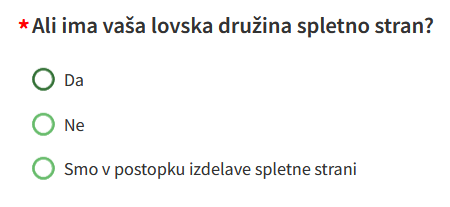
\includegraphics[width=\textwidth]{Spletno_vpra_1.png}
    \caption{Prvo vprašanje o spletnih straneh lovskih družin}
    \label{fig:spletno_vpra_1}
  \end{minipage}
  
  \vspace{0.5cm} % Adjust space between the images as needed
  
  \begin{minipage}[b]{0.8\textwidth} 
    \centering
    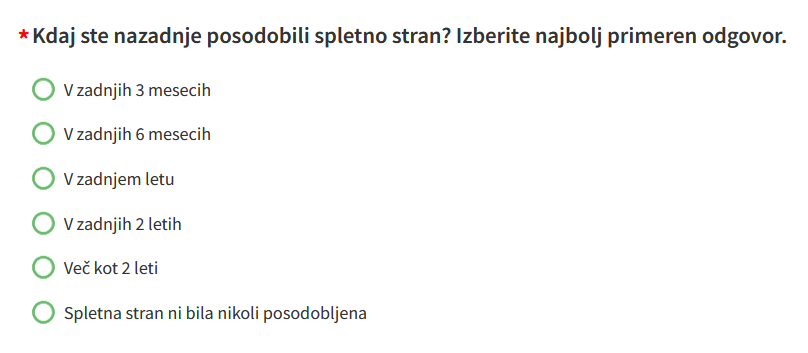
\includegraphics[width=\textwidth]{Spletno_vpra_2.png}
    \caption{Prvo pogojno vprašanje}
    \label{fig:spletno_vpra_2}
  \end{minipage}
\end{figure}

\begin{figure}[h!]  
  \centering
  \begin{minipage}[b]{\textwidth}  
    \centering
    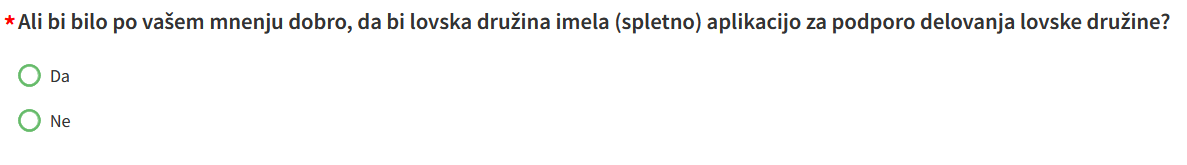
\includegraphics[width=\textwidth]{Spletno_vpra_3.png}
    \caption{Drugo splošno vprašanje o spletnih straneh lovskih družin}
    \label{fig:spletno_vpra_3}
  \end{minipage}
  
  \vspace{0.5cm} % Adjust space between the images as needed
  
  \begin{minipage}[b]{\textwidth} 
    \centering
    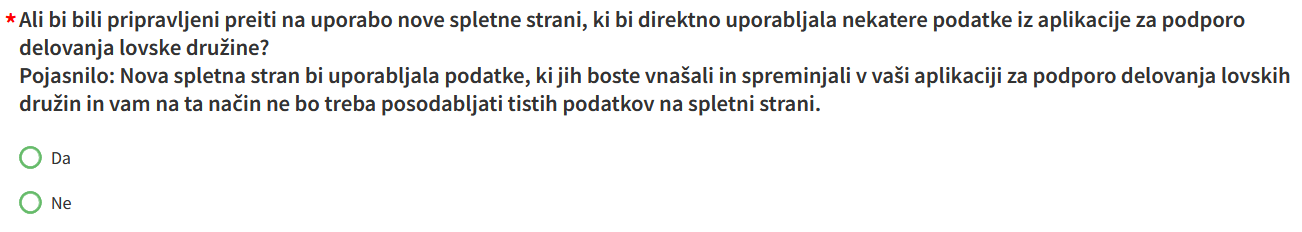
\includegraphics[width=\textwidth]{Spletno_vpra_4.png}
    \caption{Drugo pogojno vprašanje}
    \label{fig:spletno_vpra_4}
  \end{minipage}
  
\end{figure}

V prvem vprašanju nas zanima, koliko lovskih družin sploh ima spletno stran.
Če je anketiranec odgovoril, da ima njihova lovska družina spletno stran, se pojavi drugo prikazano vprašanje, ki sprašuje, kako pogosto so spletne strani posodobljene. 
S tem pridobimo bolj podrobne informacije o tem, kako pogosto se lovske družine ukvarjajo s svojimi spletnimi strani.



Pri drugem splošnem vprašanju, ki ga anketiranec dobi v vsakem primeru (ni pogojeno z odgovori prejšnjih vprašanj), je zaželeno pridobiti mnenje o pripravljenosti uporabe aplikacije za pomoč pri delovanju lovske družine.
Z odgovorom "Da" in če so pri prvem splošnem vprašanju anketiranci odgovorili, da imajo spletno stran oziroma da so v postopku izdelave spletne strani, se pojavi drugo pogojno vprašanje.
Preverja le pripravljenost predstavnikov lovskih družin, da bi omenjena aplikacija uporabljala njihove podatke.

\subsection{Vprašanja o izvajanju sestankov in izobraževanja na daljavo}

% Prva vrsta
\begin{figure}[h!]
  \centering
  \begin{minipage}[b]{\textwidth}
    \centering
    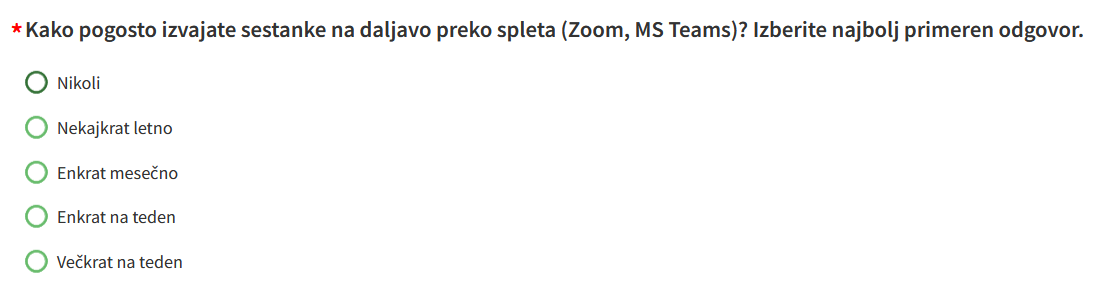
\includegraphics[width=\textwidth]{Sestanki_vpra_1.png}
    \caption{Osnovno, prvo vprašanje}
    \label{fig:sestanki_vpra_1}
  \end{minipage}
  
  \vspace{0.5cm} % Adjust space between the images as needed
  
  \begin{minipage}[b]{0.6\textwidth}
    \centering
    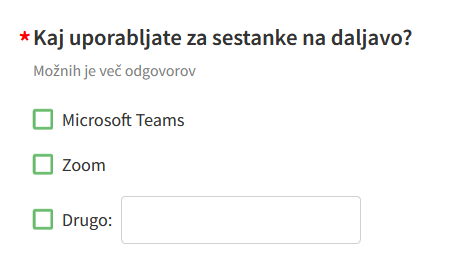
\includegraphics[width=\textwidth]{Sestanki_vpra_2.png}
    \caption{Pogojno drugo vprašanje}
    \label{fig:sestanki_vpra_2}
  \end{minipage}
\end{figure}


% Druga vrsta
\begin{figure}[h!]
  \centering
  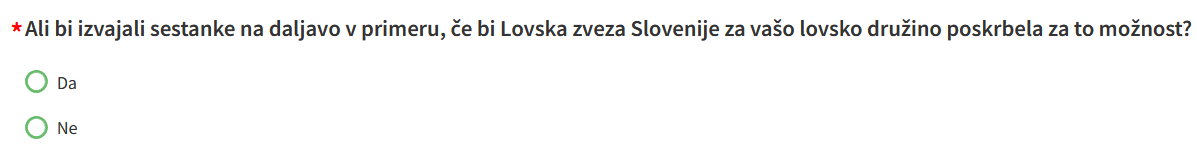
\includegraphics[width=\textwidth]{Sestanki_vpra_3.png}
  \caption{Pogojno tretje vprašanje}
  \label{fig:sestanki_vpra_3}
\end{figure}

Iz prvega vprašanja dobimo informacije o tem, kako pogosti so sestanki na daljavo v lovskih družinah.
Če anketiranec ne odgovori z "Nikoli", se pojavi drugo vprašanje, ki sprašuje o aplikacijah, s katerimi izvajajo sestanke.
V obratnem primeru pa se pojavi tretje prikazano vprašanje, ki sprašuje anketirance, ali bi spremenili svoje navade za izvajanje sestankov na daljavo, če bi za to poskrbela LZS.

\newpage
\subsection{Vprašanja o Lisjaku}

\begin{figure}[h!]
  \centering
  \begin{minipage}[b]{0.6\textwidth}
    \centering
    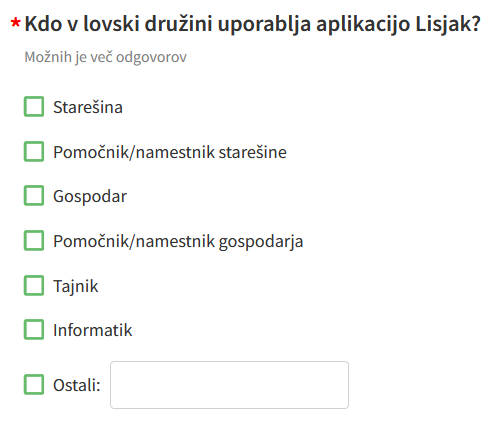
\includegraphics[width=\textwidth]{Lisjak_vpra_1.png}
    \caption{Prvo vprašanje}
    \label{fig:lisjak_vpra_1}
  \end{minipage}
  
  \vspace{0.5cm} % Adjust space between the images as needed
  
  \begin{minipage}[b]{0.7\textwidth}
    \centering
    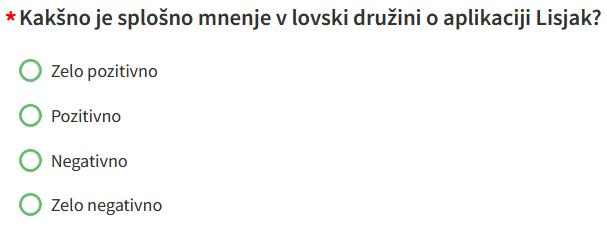
\includegraphics[width=\textwidth]{Lisjak_vpra_2.png}
    \caption{Drugo vprašanje}
    \label{fig:lisjak_vpra_2}
  \end{minipage}
\end{figure}

\begin{figure}[h!]
  \centering
  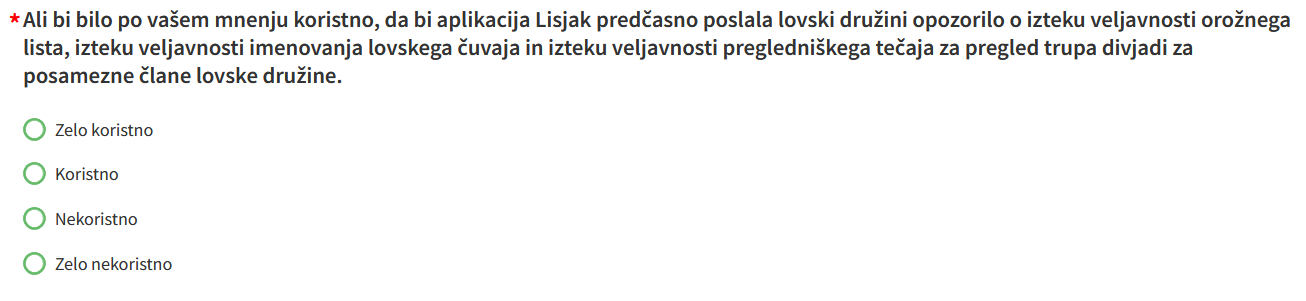
\includegraphics[width=\textwidth]{Lisjak_vpra_3.png}
  \caption{Tretje vprašanje glede sistema Lisjak}
  \label{fig:lisjak_vpra_3}
\end{figure}

Vsa tri vprašanja se pojavijo vsem izpolnjevalcem ankete, ne glede na prejšnje odgovore.
S prvim vprašanjem dobimo konkretni odgovor, kateri funkcionar v lovski družini uporablja sistem Lisjak.
Drugo vprašanje nam da splošno mnenje anketirancev o Lisjaku. 
Tretje vprašanje pa dobi informacijo, kakšna je želja lovskih družin o specifičnih problemih, s katerimi se lovske družine soočajo.
To vprašanje je bilo ustvarjeno na podlagi pogovorov s člani LZS in ZGS.
Po upokojitvi lovca ali po izteku orožnega lista mora namreč lovska družina poročati lokalni upravni enoti.
V primeru, da lovska družina ne poroča lokalni upravni enoti, so v zakonu določene denarne kazni, zato bi bilo uporabno, da bi Lisjak lovske družine vnaprej opozoril na iztek veljavnosti posameznega orožnega lista.


\begin{figure}[ht]
    \centering
    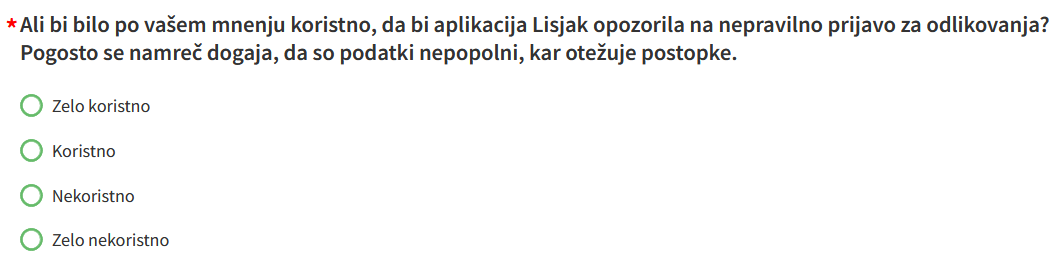
\includegraphics[width=\textwidth]{Lisjak_vpra_4.png}
    \caption{Četrto vprašanje}
\end{figure}

\begin{figure}[ht]
    \centering
    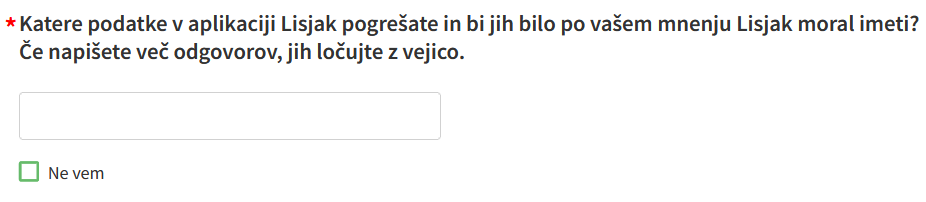
\includegraphics[width=\textwidth]{Lisjak_vpra_5.png}
    \caption{Peto vprašanje}
\end{figure}


S članom Komisije za priznanja in odlikovanja smo se pogovarjali o tem, da morajo v komisiji ročno preverjati prijave za odlikovanja.
To bi bilo možno poenostaviti s tem, da bi Lisjak sam opozoril vnašalca prijave na napake.
Četrto vprašanje zato sprašuje lovske družine, če bi jim bila taka sprememba koristna.
Peto vprašanje je namenjeno raznim predlogom lovskih družin za dodatne informacije v sistemu Lisjak.

\newpage
\subsection{Ostala vprašanja}

\begin{figure}[H]
    \centering
    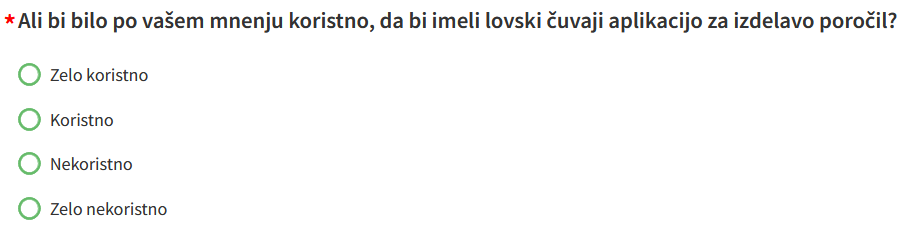
\includegraphics[width=\textwidth]{Ostalo_vpra_1.png}
    \caption{Vprašanje za čuvajsko aplikacijo}
\end{figure}


\begin{figure}[H]
    \centering
    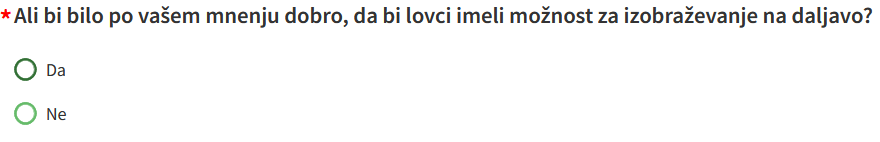
\includegraphics[width=\textwidth]{Ostalo_vpra_2.png}
    \caption{Vprašanje o lovskem izobraževanju na daljavo}
\end{figure}

\begin{figure}[H]
    \centering
    \includegraphics[width=0.8\textwidth]{Ostalo_vpra_3.png}
    \caption{Zaželene funkcije mobilne aplikacije za lovce}
\end{figure}

V prvem vprašanju smo dobili informacije lovskih družin, ali bi bila aplikacija za izdelavo poročil koristna pri delu lovskih čuvajev.
Pri drugem pa pridobimo mnenje o izobraževanju lovcev na daljavo.
Zadnje vprašanje ankete je spraševalo anketirance, katere funkcionalnosti mobilne aplikacije za lovce so zaželene.
Bila je tudi dana opcija za dodatne funkcionalnosti, kjer lahko osebe lovskih družin dajo svoje predloge.

\newpage

\section{Predstavitev in analiza rezultatov ankete}

Na anketo je odgovorilo !! predstavnikov lovskih družin, od katerih je !! končalo anketo (!! \%).
Anketa je trajala od 27. 8. 2024 do !! in anketiranci so izpolnili več kot polovico izpolnjenih anket v prvem dnevu.
Večina je izpolnila anketo preko računalnika (!! \%) ostali pa preko telefona ( !! \%).

\subsection{Rezultati vprašanj o spletnih straneh lovskih družin}

Večina lovskih družin nima svojih spletnih strani (!! \%), tiste ki jih pa imajo, jih pa večina vsaj letno posodabljajo.
Veliko anketirancev je trdilo, da bi bila aplikacija za podporo delovanja lovske družine dobra ideja in večina, ki lovskih družin, ki ima trenutno spletno stran, bi bila pripravljena preiti na uporabo nove spletne strani.

\subsection{Rezultati vprašanj o izvajanju sestankov in izobraževanja na daljavo}

Velika večina vprašanih je odgovorila, da nikoli ne izvaja sestanke na daljavo. 
Tisti redki, ki pa jih nekajkrat na leto izvajajo preko spleta, pa večinoma uporabljajo Zoom (!! \%), Microsoft Teams (!! \%), po mailu ????? (!! \%) in preko mobitela (!! \%).
To je najverjetneje zato, ker ni potrebe, saj člani lovskih družin niso zelo fizično oddaljeni.
Večina (četudi ne tako velika) tistih ki so odgovorili, da nikoli ne izvajajo sestanke preko spleta je tudi menila, da ne bi izvajala sestankov na daljavo, če bi LZS poskrbela za to možnost.
Odgovori za ponudbo za sestanke na daljavo preko LZS je pa bolj mešan.
To je lahko interpretirano tako, da je največji problem izvajanja sestankov preko spleta usklajenost posameznih članov sestanka.
Najverjetneje so pogosti problemi kot so slaba internetna povezava, nezdružljivost programske opreme in varnost razlog, da je bolj priročno, da se člani lovskih družin srečajo v živo.
Če bi pa sestanki potekali preko Lisjaka, bi bila to optimalna alternativa.


\subsection{Rezultati vprašanj o Lisjaku}

Velika večina (!! \%) anketirancev ima vsaj pozitivno splošno mnenje o Lisjaku, negativno mnenje ima le manjšina  (!! \%).
Lovski informacijski sistem deluje že skoraj dvajset let, zato je večina članov lovskih družin spoznani z njim in je navajena na delovanje.
Lisjak najbolj uporablja tajnik (!! \%), starešina (!! \%), gospodar (!! \%) in informatik (!! \%) lovske družine, pomočniki so manj omenjeni, saj najverjetneje take vloge niso prisotne pri vseh lovskih družinah.
Rezultat je seveda tudi smiseln, saj je tajništvo lovskih družin tisto, ki je zadolženo z zapiski ter uradnimi procesi ? !!.
Poleg vlog, ki so bile na voljo v anketi, je bila omenjena pogosto tudi vloga/Član kinolog.

Pri vprašanjih za predloge izboljšav Lisjaka so bili odgovori izredno pozitivni. 
Za predčasno opozorilo o izteku veljavnosti orožnega lista je le (!! \%) odgovoril, da je nekoristno, za dodajanje opozorila za odlikovanja pa tudi le (!! \%).
Iz rezultatov je možno razbrati, da je nadgradnja Lisjaka zelo dobrodošla, saj ni potrebe po prilaganju članov lovskih družin na novo programsko opremo.

Najpogostejši predlogi za dodatne podatke v informacijskem sistemu Lisjak se nanašajo na vpis in pregled podatkov o lovskih psih.
Temu so sledili dostopnost informacij za vse člane, dodatek zemljevida lovišča z lovskimi objekti, evidenca lovcev, možnost prijave škode in registracija člana ob vstopu v lovišče.
Omenjena je bila tudi splošna posodobitev Lisjaka in njegova povezava z LPN.
Bilo je tudi veliko komentarjev anketirancev, ki so trdili, da nimajo pripomb.

\subsection{Rezultati ostalih vprašanj}

Odgovori na vprašanje za možnost izobraževanja lovcev na daljavo je bilo pozitivno (!! \%).
Spletna izobrazba kot dopolnilo ali alternativa za obstoječe vrsti izobrazbe lovcev bi bila sprejeta in bi definitivno nekaterim lovcem prišla prav, še posebej najverjetneje tistim, ki so fizično oddaljeni od !! mest, kjer poteka učenje.

Velika večina anketirancev je tudi trdila, da bi bila aplikacija za izdelavo poročil koristna (!! \%). 
Le manjšina (!! \%) meni, da ne bi bilo koristno, mogoče zaradi že dobro funkcioniranih obstoječih postopkov nekaterih LD ali pa zaradi skrbi, da bi novo narejena aplikacija postala nujna za vse lovce.

Najbolj zaželena funkcionalnost anketirancev pri mobilni aplikaciji za lovce je vnos osnovnih podatkov o uplenu (!! \%).
Naslednje štiri pomembne funkcionalnosti so prikaz zasedenosti prež na zemljevidu, označitev zasedenosti in sprostitev zasedenosti preže ter vodenje dnevnika lovskega pripravnika.
Med zaželenimi funkcionalnostmi so bile omenjene lokacija uplenitve, aktualni plan odstrela, prijava oddanih strelov possameznika, evidenca vstopa v lovišče, mapa s solnicami, krmiščami, prežami...
Med ostale zaželene funkcionalnosti so bile napisane tudi pripombe, da aplikacija ni potrebna in da bo aplikacija obremenila starejše lovce oziroma, da je lov način, da se lovci odklopijo od digitalizacije. 

\chapter{Zaključek}  

Za digitalizacijo lovstva obstaja veliko nerealiziranega potenciala.
Obstoječa IT infrastruktura, vključno z LIS Lisjak, pokriva osnovne potrebe, obstajajo pa mnoge priložnosti za nadgradnjo in širšo integracijo z novonastalimi/ki niso še ustvarjeni aplikacijami/sistemi.
Uvedba osnovne platforme za elektronsko pošto in ažuriranje kontaknih podatkov je ključnega pomena za izboljšanje komunikacije med različnimi lovskimi organizacijami.
Priporočljiva je nadgradnja obstoječih sistemov, bolj kot ustvarjanjne novih sistemov, saj so skoraj vsi lovci navajeni na obstoječi sistem ter imajo starejši člani lovskih velikokrat težave pri uporabi novih digitalnih orodij.
Zaželena je tudi večja transparentnost delovanja lovskih organizacij, predvsem zaradi izobrazbe javnosti.
Za dolgoročni uspeh digitalizacije lovstva bo potrebna pripravljenost vseh deležnikov na nove priložnosti in izzive, ki jih ponuja posodobitev lovstva za 21. stoletje.
S pravilnim pristopom lahko digitalne tehnologije postanejo orodje za trajnostni razvoj, ki bo koristil lovcem in ohranjal slovensko lovsko tradicijo.


\label{end}

%%%%%%%%%%%%%%%%%%%%%%%%%%%%%%%%%%%%%%%%%%%%%%%%%%%%%%%%%%%%%%%%%%%%%%%%%%%%%%%%%%%%%%%%%%%%%%%%%%%%%%%%%%%%%%

\cleardoublepage


\printbibliography[heading=bibintoc]


\end{document}